% Options for packages loaded elsewhere
\PassOptionsToPackage{unicode}{hyperref}
\PassOptionsToPackage{hyphens}{url}
%
\documentclass[
]{book}
\usepackage{amsmath,amssymb}
\usepackage{iftex}
\ifPDFTeX
  \usepackage[T1]{fontenc}
  \usepackage[utf8]{inputenc}
  \usepackage{textcomp} % provide euro and other symbols
\else % if luatex or xetex
  \usepackage{unicode-math} % this also loads fontspec
  \defaultfontfeatures{Scale=MatchLowercase}
  \defaultfontfeatures[\rmfamily]{Ligatures=TeX,Scale=1}
\fi
\usepackage{lmodern}
\ifPDFTeX\else
  % xetex/luatex font selection
\fi
% Use upquote if available, for straight quotes in verbatim environments
\IfFileExists{upquote.sty}{\usepackage{upquote}}{}
\IfFileExists{microtype.sty}{% use microtype if available
  \usepackage[]{microtype}
  \UseMicrotypeSet[protrusion]{basicmath} % disable protrusion for tt fonts
}{}
\makeatletter
\@ifundefined{KOMAClassName}{% if non-KOMA class
  \IfFileExists{parskip.sty}{%
    \usepackage{parskip}
  }{% else
    \setlength{\parindent}{0pt}
    \setlength{\parskip}{6pt plus 2pt minus 1pt}}
}{% if KOMA class
  \KOMAoptions{parskip=half}}
\makeatother
\usepackage{xcolor}
\usepackage{color}
\usepackage{fancyvrb}
\newcommand{\VerbBar}{|}
\newcommand{\VERB}{\Verb[commandchars=\\\{\}]}
\DefineVerbatimEnvironment{Highlighting}{Verbatim}{commandchars=\\\{\}}
% Add ',fontsize=\small' for more characters per line
\usepackage{framed}
\definecolor{shadecolor}{RGB}{248,248,248}
\newenvironment{Shaded}{\begin{snugshade}}{\end{snugshade}}
\newcommand{\AlertTok}[1]{\textcolor[rgb]{0.94,0.16,0.16}{#1}}
\newcommand{\AnnotationTok}[1]{\textcolor[rgb]{0.56,0.35,0.01}{\textbf{\textit{#1}}}}
\newcommand{\AttributeTok}[1]{\textcolor[rgb]{0.13,0.29,0.53}{#1}}
\newcommand{\BaseNTok}[1]{\textcolor[rgb]{0.00,0.00,0.81}{#1}}
\newcommand{\BuiltInTok}[1]{#1}
\newcommand{\CharTok}[1]{\textcolor[rgb]{0.31,0.60,0.02}{#1}}
\newcommand{\CommentTok}[1]{\textcolor[rgb]{0.56,0.35,0.01}{\textit{#1}}}
\newcommand{\CommentVarTok}[1]{\textcolor[rgb]{0.56,0.35,0.01}{\textbf{\textit{#1}}}}
\newcommand{\ConstantTok}[1]{\textcolor[rgb]{0.56,0.35,0.01}{#1}}
\newcommand{\ControlFlowTok}[1]{\textcolor[rgb]{0.13,0.29,0.53}{\textbf{#1}}}
\newcommand{\DataTypeTok}[1]{\textcolor[rgb]{0.13,0.29,0.53}{#1}}
\newcommand{\DecValTok}[1]{\textcolor[rgb]{0.00,0.00,0.81}{#1}}
\newcommand{\DocumentationTok}[1]{\textcolor[rgb]{0.56,0.35,0.01}{\textbf{\textit{#1}}}}
\newcommand{\ErrorTok}[1]{\textcolor[rgb]{0.64,0.00,0.00}{\textbf{#1}}}
\newcommand{\ExtensionTok}[1]{#1}
\newcommand{\FloatTok}[1]{\textcolor[rgb]{0.00,0.00,0.81}{#1}}
\newcommand{\FunctionTok}[1]{\textcolor[rgb]{0.13,0.29,0.53}{\textbf{#1}}}
\newcommand{\ImportTok}[1]{#1}
\newcommand{\InformationTok}[1]{\textcolor[rgb]{0.56,0.35,0.01}{\textbf{\textit{#1}}}}
\newcommand{\KeywordTok}[1]{\textcolor[rgb]{0.13,0.29,0.53}{\textbf{#1}}}
\newcommand{\NormalTok}[1]{#1}
\newcommand{\OperatorTok}[1]{\textcolor[rgb]{0.81,0.36,0.00}{\textbf{#1}}}
\newcommand{\OtherTok}[1]{\textcolor[rgb]{0.56,0.35,0.01}{#1}}
\newcommand{\PreprocessorTok}[1]{\textcolor[rgb]{0.56,0.35,0.01}{\textit{#1}}}
\newcommand{\RegionMarkerTok}[1]{#1}
\newcommand{\SpecialCharTok}[1]{\textcolor[rgb]{0.81,0.36,0.00}{\textbf{#1}}}
\newcommand{\SpecialStringTok}[1]{\textcolor[rgb]{0.31,0.60,0.02}{#1}}
\newcommand{\StringTok}[1]{\textcolor[rgb]{0.31,0.60,0.02}{#1}}
\newcommand{\VariableTok}[1]{\textcolor[rgb]{0.00,0.00,0.00}{#1}}
\newcommand{\VerbatimStringTok}[1]{\textcolor[rgb]{0.31,0.60,0.02}{#1}}
\newcommand{\WarningTok}[1]{\textcolor[rgb]{0.56,0.35,0.01}{\textbf{\textit{#1}}}}
\usepackage{longtable,booktabs,array}
\usepackage{calc} % for calculating minipage widths
% Correct order of tables after \paragraph or \subparagraph
\usepackage{etoolbox}
\makeatletter
\patchcmd\longtable{\par}{\if@noskipsec\mbox{}\fi\par}{}{}
\makeatother
% Allow footnotes in longtable head/foot
\IfFileExists{footnotehyper.sty}{\usepackage{footnotehyper}}{\usepackage{footnote}}
\makesavenoteenv{longtable}
\usepackage{graphicx}
\makeatletter
\def\maxwidth{\ifdim\Gin@nat@width>\linewidth\linewidth\else\Gin@nat@width\fi}
\def\maxheight{\ifdim\Gin@nat@height>\textheight\textheight\else\Gin@nat@height\fi}
\makeatother
% Scale images if necessary, so that they will not overflow the page
% margins by default, and it is still possible to overwrite the defaults
% using explicit options in \includegraphics[width, height, ...]{}
\setkeys{Gin}{width=\maxwidth,height=\maxheight,keepaspectratio}
% Set default figure placement to htbp
\makeatletter
\def\fps@figure{htbp}
\makeatother
\setlength{\emergencystretch}{3em} % prevent overfull lines
\providecommand{\tightlist}{%
  \setlength{\itemsep}{0pt}\setlength{\parskip}{0pt}}
\setcounter{secnumdepth}{5}
\ifLuaTeX
  \usepackage{selnolig}  % disable illegal ligatures
\fi
\usepackage[]{natbib}
\bibliographystyle{apalike}
\usepackage{bookmark}
\IfFileExists{xurl.sty}{\usepackage{xurl}}{} % add URL line breaks if available
\urlstyle{same}
\hypersetup{
  pdftitle={Genome polarisation with diemr},
  pdfauthor={Natália Martínková},
  hidelinks,
  pdfcreator={LaTeX via pandoc}}

\title{Genome polarisation with diemr}
\author{Natália Martínková}
\date{Last updated: 2025-10-15}

\begin{document}
\maketitle

{
\setcounter{tocdepth}{1}
\tableofcontents
}
\chapter{Introduction}\label{introduction}

Genome polarisation is a genome-painting approach based on the likelihood-based diagnostic index expectation maximisation (\emph{diem}) algorithm \citep{Baird2023}. It identifies which alleles of single-nucleotide variants (SNV) belong to either side of a barrier to gene flow, co-estimating both the assignment of individuals to a barrier side and the diagnosticity of each marker, meaning how consistently individuals on one side are homozygous for the allele associated with that side.

By inferring which parts of the genome correspond to each parental lineage, genome polarisation provides a direct view of \textbf{how barriers to gene flow shape genomic architecture}. It can detect and quantify hybridisation, distinguish introgressed from non-introgressed regions, and reveal how species boundaries evolve during speciation and diversification. Compared with methods such as STRUCTURE, ADMIXTURE, or PCA, which summarise population structure statistically, genome polarisation explicitly identifies the genomic segments that define the divergence between taxa or lineages.

The diagnostic index computed by \emph{diem} \textbf{highlights markers that are most informative} for the primary axis of genetic differentiation. These diagnostic loci can then be used to describe patterns of hybridisation, assess barrier strength, or visualise the genomic distribution of ancestry.

This book provides a step-by-step guide to performing genome polarisation analyses in \texttt{R} using \href{https://github.com/nmartinkova/diemr}{the \texttt{diemr} package}, also available from \href{https://CRAN.R-project.org/package=diemr}{CRAN}. The package includes functions for input validation, file-format conversion, visualisation, and diagnostic summaries, with examples based on typical genomic datasets such as variant call format (VCF) files and SNP matrices. By the end of the book, users will be able to run the complete analysis workflow, interpret its outputs, and generate graphical representations of genome polarisation.

The \emph{diem} algorithm itself is also implemented in \texttt{Mathematica} and \texttt{Python}, available \href{https://github.com/StuartJEBaird/diem}{here}, allowing reproducibility and interoperability across analytical environments.

\section{How to cite}\label{how-to-cite}

If you use the \emph{diemr} package or this documentation in your work, please cite:

Baird, S. J. E., J. Petružela, I. Jaroň, P. Škrabánek, and N. Martínková. 2023. \emph{Genome polarisation for detecting barriers to geneflow.} Methods in Ecology and Evolution 14: 512--28. \url{https://doi.org/10.1111/2041-210X.14010}.

and this online documentation for the \texttt{diemr} package:

Martínková, N. 2025. \emph{Genome polarisation with diemr.} Bookdown online documentation. Available at: \url{https://nmartinkova.github.io/genome-polarisation/}.

\chapter{Quick start}\label{intro}

\emph{Natália Martínková and Stuart J. E. Baird}

The package \texttt{diemr} incorporates the diagnostic index expectation maximisation algorithm used to
estimate which genomic alleles belong to which side of a barrier to geneflow. To start
using \texttt{diemr}, load the package or install it from CRAN if it is not yet available:

\begin{Shaded}
\begin{Highlighting}[]
\CommentTok{\# Attempt to load a package, if the package was not available, install and load}
\ControlFlowTok{if}\NormalTok{(}\SpecialCharTok{!}\FunctionTok{require}\NormalTok{(}\StringTok{"diemr"}\NormalTok{, }\AttributeTok{character.only =} \ConstantTok{TRUE}\NormalTok{))\{}
    \FunctionTok{install.packages}\NormalTok{(}\StringTok{"diemr"}\NormalTok{, }\AttributeTok{dependencies =} \ConstantTok{TRUE}\NormalTok{)}
    \FunctionTok{library}\NormalTok{(}\StringTok{"diemr"}\NormalTok{, }\AttributeTok{character.only =} \ConstantTok{TRUE}\NormalTok{)}
\NormalTok{\}}
\end{Highlighting}
\end{Shaded}

Next, assemble paths to all files containing the data to be used by \texttt{diemr}.
Here, we will use a tiny example dataset that is included in the package for illustrating
the analysis workflow. A good practice is to check that all files contain data in the
correct format for all individuals and markers. Additionally, the analysis will need a
list with \textbf{ploidies for all genomic compartments and individuals}, and a vector with
\textbf{indices of samples} that will be included in the analysis.

\begin{Shaded}
\begin{Highlighting}[]
\NormalTok{filepaths }\OtherTok{\textless{}{-}} \FunctionTok{system.file}\NormalTok{(}\StringTok{"extdata"}\NormalTok{, }\StringTok{"data7x3.txt"}\NormalTok{, }\AttributeTok{package =} \StringTok{"diemr"}\NormalTok{)}
\CommentTok{\# Analysing six individuals}
\NormalTok{samples }\OtherTok{\textless{}{-}} \DecValTok{1}\SpecialCharTok{:}\DecValTok{6}
\CommentTok{\# Assuming diploid markers of all individuals}
\NormalTok{ploidies }\OtherTok{=} \FunctionTok{rep}\NormalTok{(}\FunctionTok{list}\NormalTok{(}\FunctionTok{rep}\NormalTok{(}\DecValTok{2}\NormalTok{, }\FunctionTok{nchar}\NormalTok{(}\FunctionTok{readLines}\NormalTok{(filepaths[}\DecValTok{1}\NormalTok{])[}\DecValTok{1}\NormalTok{]) }\SpecialCharTok{{-}} \DecValTok{1}\NormalTok{)), }\FunctionTok{length}\NormalTok{(filepaths))}
\FunctionTok{CheckDiemFormat}\NormalTok{(}\AttributeTok{files =}\NormalTok{ filepaths, }
                \AttributeTok{ChosenInds =}\NormalTok{ samples,}
                \AttributeTok{ploidy =}\NormalTok{ ploidies)}
\CommentTok{\# File check passed: TRUE}
\CommentTok{\# Ploidy check passed: TRUE}
\end{Highlighting}
\end{Shaded}

If the \texttt{CheckDiemFormat()} function fails, work through the error messages and fix
the stored input files accordingly. The algorithm repeatedly accesses data from the
harddisk, so seeing the passed file and variable check prior to the analysis is critical.

To estimate the marker polarities, their diagnostic indices and support, run the function
\texttt{diem()} with default settings. Here, we have only one file with data, so paralelisation
is unnecessary, and we set \texttt{nCores\ =\ 1}. \textbf{The Windows operating system only allows for
nCores = 1}. Other operating systems can process multiple genomic compartments (e.g.~
chromosomes) in parallel, the analysis of different genomic compartment files running on
multiple processors.

\begin{Shaded}
\begin{Highlighting}[]
\NormalTok{res }\OtherTok{\textless{}{-}} \FunctionTok{diem}\NormalTok{(}\AttributeTok{files =}\NormalTok{ filepaths, }
            \AttributeTok{ploidy =}\NormalTok{ ploidies, }
            \AttributeTok{markerPolarity =} \FunctionTok{list}\NormalTok{(}\FunctionTok{c}\NormalTok{(}\ConstantTok{FALSE}\NormalTok{, }\ConstantTok{FALSE}\NormalTok{, }\ConstantTok{TRUE}\NormalTok{)),}
            \AttributeTok{ChosenInds =}\NormalTok{ samples, }
            \AttributeTok{nCores =} \DecValTok{1}\NormalTok{)}
\end{Highlighting}
\end{Shaded}

The result is a list, where the element \texttt{res\$DI} contains a table with marker
polarities, their diagnostic indices and support.

\begin{Shaded}
\begin{Highlighting}[]
\NormalTok{res}\SpecialCharTok{$}\NormalTok{DI}
\CommentTok{\#   newPolarity         DI   Support Marker}
\CommentTok{\# 1       FALSE  {-}4.872256 15.930181      1}
\CommentTok{\# 2        TRUE  {-}3.520647 18.633399      2}
\CommentTok{\# 3        TRUE {-}13.274822  6.130625      3}
\end{Highlighting}
\end{Shaded}

The column \texttt{newPolarity} means that marker 1 should be imported for subsequent
analyses as is, and markers 2 and 3 should be imported with 0 replaced with 2 and 2
replaced with 0 (hereafter `flipped' \(0 \leftrightarrow 2\)). The marker 3 has the lowest diagnostic
index and low support, indicating
that the genotypes scored at this marker are poorly related to the barrier to geneflow
arbitrated by the data.

With the marker polarities optimised to detect a barrier to geneflow, a plot of the
polarised genome will show how genomic regions cross the barrier. First, the genotypes
need to be imported with optimal marker polarities. Second, individual hybrid indices
need to be calculated from the polarised genotypes. And last, the data will be plotted
as a raster image.

\begin{Shaded}
\begin{Highlighting}[]
\NormalTok{genotypes }\OtherTok{\textless{}{-}} \FunctionTok{importPolarized}\NormalTok{(}\AttributeTok{file =}\NormalTok{ filepaths, }
                             \AttributeTok{changePolarity =}\NormalTok{ res}\SpecialCharTok{$}\NormalTok{markerPolarity, }
                             \AttributeTok{ChosenInds =}\NormalTok{ samples)}
                             
\NormalTok{HI }\OtherTok{\textless{}{-}} \FunctionTok{hybridIndex}\NormalTok{(res}\SpecialCharTok{$}\NormalTok{I4)}
           
\FunctionTok{plotPolarized}\NormalTok{(}\AttributeTok{genotypes =}\NormalTok{ genotypes,}
              \AttributeTok{HI =}\NormalTok{ HI[samples])}
\end{Highlighting}
\end{Shaded}

\begin{center}
\includegraphics{01-diemr-diagnostic-index-expecation-maximisation-in-r_files/figure-latex/unnamed-chunk-5-1} \end{center}

\textbf{CAUTION:} This is just a \emph{quick start} to get you started! For real datasets you will use the diagnostic index (DI) to filter the full set of sites you have analysed with \texttt{diem} in order to plot only those markers relevant to any barrier detected in the analysis. See \textbf{Chapter \ref{DIfiltering}} for guidelines.

\chapter{Input data}\label{diemFormat}

\emph{Natália Martínková and Stuart J. E. Baird}

The \texttt{diemr} package uses a consise genome representation. Let's have a small dataset
of three markers genotyped for seven individuals.

\begin{Shaded}
\begin{Highlighting}[]
\NormalTok{S0011222}
\NormalTok{S1210001}
\NormalTok{S02221U0}
\end{Highlighting}
\end{Shaded}

The genotypes encoded as \texttt{0} represent homozygotes for an allele attributed to barrier side A, \texttt{1} are
heterozygous genotypes, \texttt{2} are homozygotes for another allele, attributed to barrier side B, and \texttt{U}
(symbol ``\_'' is also allowed) represents an unknown state or a third (fourth) allele. The power of
\texttt{diem} lies in the assurance that the user does not need to determine the true assignment to barrier sides A and B before the analysis and the specific genotypes encoded as \texttt{0} and \texttt{2} respectively
can be arbitrary.

The leading \texttt{S} on each line of the input file is ensures that the marker genotypes are
read in as a string on all operating systems. The \texttt{S} is dropped during import of the genotypes, and
the dataset is imported as a character matrix of all sites.

\section{Multiple compartments with different ploidies}\label{multiple-compartments-with-different-ploidies}

Some genomic compartments differ between individuals in their ploidy. For example, markers located on
chromosome X in mammals will be diploid in females, but haploid in males. Ploidy differences between
individuals influence calculation of the hybrid index, which in turn has an effect on the \emph{diem} analysis.

To set up the \emph{diem} analysis with multiple compartments, the markers with different individual ploidies
must be stored in separate files. The file analysed in the \hyperref[intro]{\textbf{Quick start}} chapter could contain
markers from autosomes and an additional file will contain markers from an X
chromosome, with individuals 2 and 6 being males. The respective ploidies for the second genomic
compartment
will be \texttt{c(2,\ 1,\ 2,\ 2,\ 2,\ 1,\ 2)}.

Arguments \texttt{files} and \texttt{ploidy} will need to reflect the information, taking care that the order of filenames
corresponds to the order of elements in the list of ploidies. \texttt{diem} cannot check that the order of the
elements
is correct, only that the information is in the correct format.

\begin{Shaded}
\begin{Highlighting}[]
\NormalTok{filepaths2 }\OtherTok{\textless{}{-}} \FunctionTok{c}\NormalTok{(}\FunctionTok{system.file}\NormalTok{(}\StringTok{"extdata"}\NormalTok{, }\StringTok{"data7x3.txt"}\NormalTok{, }\AttributeTok{package =} \StringTok{"diemr"}\NormalTok{),}
                \FunctionTok{system.file}\NormalTok{(}\StringTok{"extdata"}\NormalTok{, }\StringTok{"data7x10.txt"}\NormalTok{, }\AttributeTok{package =} \StringTok{"diemr"}\NormalTok{))}
               
\NormalTok{ploidies2 }\OtherTok{\textless{}{-}} \FunctionTok{list}\NormalTok{(}\FunctionTok{rep}\NormalTok{(}\DecValTok{2}\NormalTok{, }\DecValTok{7}\NormalTok{),}
                  \FunctionTok{c}\NormalTok{(}\DecValTok{2}\NormalTok{, }\DecValTok{1}\NormalTok{, }\DecValTok{2}\NormalTok{, }\DecValTok{2}\NormalTok{, }\DecValTok{2}\NormalTok{, }\DecValTok{1}\NormalTok{, }\DecValTok{2}\NormalTok{))}

\FunctionTok{CheckDiemFormat}\NormalTok{(}\AttributeTok{files =}\NormalTok{ filepaths2, }
                \AttributeTok{ChosenInds =}\NormalTok{ samples,}
                \AttributeTok{ploidy =}\NormalTok{ ploidies2)}
\CommentTok{\# File check passed: TRUE}
\CommentTok{\# Ploidy check passed: TRUE}

\CommentTok{\# Set random seed for repeatibility of null polarities (optional)}
\FunctionTok{set.seed}\NormalTok{(}\DecValTok{39583782}\NormalTok{)}

\CommentTok{\# Run diem }
\NormalTok{res2 }\OtherTok{\textless{}{-}} \FunctionTok{diem}\NormalTok{(}\AttributeTok{files =}\NormalTok{ filepaths2, }
             \AttributeTok{ploidy =}\NormalTok{ ploidies2, }
             \AttributeTok{markerPolarity =} \ConstantTok{FALSE}\NormalTok{,}
             \AttributeTok{ChosenInds =}\NormalTok{ samples, }
             \AttributeTok{nCores =} \DecValTok{1}\NormalTok{)}
\end{Highlighting}
\end{Shaded}

Plotting polarised genomes from multiple compartments requires separate import of the compartment data.
The polarities in the \texttt{res2\$markerPolarity} element are combined across all compartments, and extracting
them requires knowledge of the number of markers in each compartment. Alternatively, the marker polarities
from each compartment can be extracted from the list in the \texttt{res2\$PolarityChanges} element.

\begin{Shaded}
\begin{Highlighting}[]
\CommentTok{\# Import each compartment into a list}
\NormalTok{genotypes2 }\OtherTok{\textless{}{-}} \FunctionTok{importPolarized}\NormalTok{(}\AttributeTok{file =}\NormalTok{ filepaths2, }
                       \AttributeTok{changePolarity =}\NormalTok{ res2}\SpecialCharTok{$}\NormalTok{markerPolarity, }
                       \AttributeTok{ChosenInds =}\NormalTok{ samples)}\ErrorTok{)} 
                       
\CommentTok{\# Load individual hybrid indices from a stored file}
\NormalTok{h2 }\OtherTok{\textless{}{-}} \FunctionTok{hybridIndex}\NormalTok{(}\StringTok{"HIwithOptimalPolarities.txt"}\NormalTok{)}

\CommentTok{\# Plot the polarised genotypes}
\FunctionTok{plotPolarized}\NormalTok{(}\AttributeTok{genotypes =}\NormalTok{ genotypes2,}
              \AttributeTok{HI =}\NormalTok{ h2[samples])}
\end{Highlighting}
\end{Shaded}

\begin{center}
\includegraphics{01-diemr-diagnostic-index-expecation-maximisation-in-r_files/figure-latex/unnamed-chunk-9-1} \end{center}

\chapter{Importing data for genome polarisation}\label{importing-data-for-genome-polarisation}

\emph{Natália Martínková and Stuart J. E. Baird}

\section{Conversion from VCF format}\label{conversion-from-vcf-format}

The package \texttt{diemr} provides a function \texttt{vcf2diem}, which converts diploid genotypes in a vcf file (optionally, the vcf file can be gzipped) or an \texttt{vcfR} object loaded into \texttt{R} to a file with format required by \texttt{diem}. To start, load the \texttt{diemr} package or install it from CRAN if it is not yet available:

\begin{Shaded}
\begin{Highlighting}[]
\CommentTok{\# Attempt to load a package, if the package was not }
\CommentTok{\# available, install and load}
\ControlFlowTok{if}\NormalTok{(}\SpecialCharTok{!}\FunctionTok{require}\NormalTok{(}\StringTok{"diemr"}\NormalTok{, }\AttributeTok{character.only =} \ConstantTok{TRUE}\NormalTok{))\{}
    \FunctionTok{install.packages}\NormalTok{(}\StringTok{"diemr"}\NormalTok{, }\AttributeTok{dependencies =} \ConstantTok{TRUE}\NormalTok{)}
    \FunctionTok{library}\NormalTok{(}\StringTok{"diemr"}\NormalTok{, }\AttributeTok{character.only =} \ConstantTok{TRUE}\NormalTok{)}
\NormalTok{\}}
\end{Highlighting}
\end{Shaded}

Next, decide whether all markers in the vcf file should be polarised from one file, or whether the analysis will benefit from parallelisation. Parallelisation is available on UNIX-based platforms, and we advise to use it for large datasets. \texttt{diem} itself can also work in parallel on multiple data \emph{compartments}. vcf files and \emph{compartments} can correspond to the same thing OR you can concatenate/split vcf2diem outputs to produce \texttt{diem} input \emph{compartments}.

\begin{Shaded}
\begin{Highlighting}[]
\CommentTok{\# Path to the vcf file}
\NormalTok{inputfile }\OtherTok{\textless{}{-}} \FunctionTok{system.file}\NormalTok{(}\StringTok{"extdata"}\NormalTok{, }\StringTok{"myotis.vcf"}\NormalTok{, }\AttributeTok{package =} \StringTok{"diemr"}\NormalTok{)}
\CommentTok{\# File name for the output}
\CommentTok{\# If working directory does not have writing privileges, }
\CommentTok{\# the filename must include a path to a suitable folder}
\NormalTok{outputfile }\OtherTok{\textless{}{-}} \StringTok{"myotis"}
\CommentTok{\# Convert the vcf file to two diem files}
\FunctionTok{vcf2diem}\NormalTok{(}\AttributeTok{SNP =}\NormalTok{ inputfile, }\AttributeTok{filename =}\NormalTok{ outputfile, }\AttributeTok{chunk =} \DecValTok{2}\NormalTok{)}
\CommentTok{\# Expecting to include 11 markers per diem file.}
\CommentTok{\# If you expect more markers in the file, provide suitable chunk size.}
\CommentTok{\# Done with chunk 1}
\end{Highlighting}
\end{Shaded}

The \texttt{vcf2diem} function processes calls for sites into the \texttt{diem} encoding for sites. The site order will be identical to that in the original vcf file (but see chapter \hyperref[sites-not-informative-for-genome-polarisation]{Sites not informative for genome polarisation}).

\section{Principle of conversion to diem format}\label{principle-of-conversion-to-diem-format}

The \texttt{diemr} package uses a concise genome representation, differentiating homozygotes for the two most frequent alleles at each site, and their respective heterozygotes (mixed state of the two most common alleles). All other genotypes represent an unknown state. Specifically, the genotypes encoded as \texttt{0} represent homozygotes for one of the two most frequent alleles,
\texttt{1} are heterozygous (mixed state) genotypes for the two most frequent alleles,
\texttt{2} are homozygotes for the other allele,
and \texttt{U} (symbol ``\_'' is also allowed) is an unknown state that can be a missing genotype or a genotype that includes a third (or a fourth) allele.

\subsection{Invariant sites and indels}\label{invariant-sites-and-indels}

What logically follows from this description is that genome polarisation is meaningful only for variant sites (markers). Invariant sites will have \textbf{low support} and, though they will not change the \texttt{diem} outcome, they will slow down convergence and obscure the nature of change between taxa. During \texttt{diem} iterations their obscuring effect is removed by rescaling the hybrid indices onto \([0,1]\)

Including invariant sites in genome polarisation is acceptable, and likely unavoidable. A proportion of truly invariant sites will be mis-diagnosed as variant due to sequencing errors.

At this time, genome polarisation uses variant markers where alleles differ in nucleotide substitutions. Insertions or deletions (indels) are not allowed to be classified among the most frequent alleles in the \texttt{vcf2diem} function.

\subsection{Sites not informative for genome polarisation}\label{sites-not-informative-for-genome-polarisation}

Along side invariant sites, some variant sites are also uninformative for genome polarisation. Sites that include only missing data and heterozygous genotypes are unpolarisable. In general applications, one might wish to exclude sites that are only included in a \texttt{vcf} due to the presence of a single heterozygous individual.

Uninformative sites will have support equal to 0, and their polarity will thus be equal to the null polarity. Including uninformative sites has similar consequences to including invariant sites. When a user wishes to retain such sites, we advice to then filter polarised markers with high support (or simply high diagnostic index, which is strongly correlated with support) for subsequent analyses and interpretation.

\subsection{Haploid data}\label{haploid-data}

Haploid data, including markers on sex chromosomes of the heterogametic sex, are usually shown as sequence alignments. To illustrate the principle of genome representation used in \texttt{diem}, let's have an 8bp-long alignment with five individuals.

\begin{Shaded}
\begin{Highlighting}[]
\DecValTok{5} \DecValTok{8}
\NormalTok{ind1   AACCTTGG}
\NormalTok{ind2   TACGATGG}
\NormalTok{ind3   TACC}\SpecialCharTok{{-}}\NormalTok{TGT}
\NormalTok{ind4   CACGTTGG}
\NormalTok{ind5   AACCTTGT}
\end{Highlighting}
\end{Shaded}

We can see that the example alignment contains four variant markers at sites 1, 4, 5, and 8. Marker 5 contains a deletion in ind3, while other markers vary in different nucleotide substitutions. In marker 1, two individuals have an allele A, two individuals have an allele T and one has a C. This marker can be resolved in terms of two most frequent alleles A and T, where the individual ind4 has a third allele and is therefore considered as having an unknown genomic state. To convert the marker into \texttt{diem} format, we must make a decision on which allele will be encoded as 0. The choice is arbitrary. Good practice is to \textbf{keep a record of genotype encoding}. Let's decide that all alleles in ind1 will be encoded as 0. Marker 1 will then be \texttt{022\_0}.

Contrary to DNA sequence alignments, diem format transposes the data. Rows in diem input files are markers and columns represent individual samples. The diem output for the example alignment will thus have four lines representing the four variant markers, and five columns representing the individuals.

\begin{Shaded}
\begin{Highlighting}[]
\NormalTok{Marker1   }\DecValTok{022}\NormalTok{\_0}
\NormalTok{Marker4   }\DecValTok{02020}
\NormalTok{Marker5   }\DecValTok{02}\NormalTok{\_00}
\NormalTok{Marker8   }\DecValTok{00202}
\end{Highlighting}
\end{Shaded}

The diem format does not store information on marker identification or location. This metadata must be saved separately in a `bed-like' file (with at minimum the scaffold and position for each site). \texttt{diem} uses a prefix \texttt{S} at line starts to ensure that all operating systems always read genotypes as strings without attempting to convert them into numbers. Encoding of markers 4 and 8 shown above is at risk of being interpreted as numeric. The final file in \texttt{diem} format will be:

\begin{Shaded}
\begin{Highlighting}[]
\NormalTok{S022\_0}
\NormalTok{S02020}
\NormalTok{S02\_00}
\NormalTok{S00202}
\end{Highlighting}
\end{Shaded}

\subsection{Diploid data}\label{diploid-data}

\subsubsection{Heterozygotes in DNA sequence alignments}\label{heterozygotes-in-dna-sequence-alignments}

Diploid markers in DNA sequence alignment can be resolved in an analogous way to haploid markers. Heterozygotes in alignments can be identified according to their \href{https://www.ncbi.nlm.nih.gov/pmc/articles/PMC2865858/table/T1/}{IUPAC DNA ambiguity codes}. For example, code W may represent an accepted heterozygote in Marker 1, where the most frequent alleles are A and T.

\section{Variant call format}\label{variant-call-format}

Variant markers in genomic context will be most often identified using variant callers from sequence reads mapped onto a reference. Such data are stored or can be converted to variant call format (vcf). We implemented conversion of vcf files to diem format for the \href{https://github.com/samtools/hts-specs/blob/master/VCFv4.2.pdf}{vcf version 4.2} in function \texttt{vcf2diem}. The function resolves indels and markers with more than two alleles to obtain biallelic genotypes for all markers included in the original vcf file.

\begin{enumerate}
\def\labelenumi{\arabic{enumi}.}
\tightlist
\item
  Markers with the reference allele (column REF) containing insertions are set as unknown.
\item
  Markers with the alternative allele (column ALT) containing only indels are set as unknown.
\item
  Indels in the alternative alleles are set as unknown.
\item
  Overall allele counts in markers with more than two alleles representing substitutions are calculated and the two most frequent alleles are selected. Ties are (arbitrarily) resolved according to the allele order in the vcf file.
\item
  Third and fourth most frequent substitutions are set as unknown.
\end{enumerate}

The conversion might result in some markers no longer being polymorphic. We advise checking how frequent invariant markers are after conversion.

\begin{Shaded}
\begin{Highlighting}[]
\CommentTok{\# Import the first converted file for all individuals }
\CommentTok{\# and without changing marker polarity}
\NormalTok{myotis }\OtherTok{\textless{}{-}} \FunctionTok{importPolarized}\NormalTok{(}\StringTok{"myotis{-}01.txt"}\NormalTok{, }
                          \AttributeTok{changePolarity =} \FunctionTok{rep}\NormalTok{(}\ConstantTok{FALSE}\NormalTok{, }\DecValTok{11}\NormalTok{), }
                          \AttributeTok{ChosenInds =} \DecValTok{1}\SpecialCharTok{:}\DecValTok{14}\NormalTok{)}
\CommentTok{\# Check whether a marker includes heterozygotes }
\CommentTok{\# or that there is more than one genotype}
\FunctionTok{apply}\NormalTok{(myotis, }\AttributeTok{MARGIN =} \DecValTok{2}\NormalTok{, }
      \AttributeTok{FUN =}\NormalTok{ \textbackslash{}(x) }\FunctionTok{any}\NormalTok{(}\FunctionTok{grepl}\NormalTok{(}\StringTok{"1"}\NormalTok{, x)) }\SpecialCharTok{|} \FunctionTok{sum}\NormalTok{(}\FunctionTok{levels}\NormalTok{(}\FunctionTok{factor}\NormalTok{(x)) }\SpecialCharTok{\%in\%} \FunctionTok{c}\NormalTok{(}\StringTok{"0"}\NormalTok{, }\StringTok{"1"}\NormalTok{, }\StringTok{"2"}\NormalTok{)) }\SpecialCharTok{\textgreater{}} \DecValTok{1}\NormalTok{) }
\CommentTok{\#    m1    m2    m3    m4    m5    m6    m7    m8    m9   m10   m11 }
\CommentTok{\# FALSE FALSE FALSE FALSE  TRUE  TRUE  TRUE  TRUE  TRUE  TRUE  TRUE }
\end{Highlighting}
\end{Shaded}

Starting from version 1.2.2, \texttt{vcf2diem} removes markers that include

\begin{enumerate}
\def\labelenumi{\arabic{enumi}.}
\tightlist
\item
  only missing data and heterozygotes,
\item
  missing data, homozygotes for the most frequent allele and one heterozygote,
\item
  missing data, homozygotes for one ALT allele and one heterozygote.
\end{enumerate}

We include a list of the removed markers in a bed-like file ending with \emph{-includedSites.txt} in the working directory. The file includes information from columns \texttt{CHROM}, \texttt{POS}, and \texttt{QUAL} for the respective markers, and records the (good practice) \textbf{record of genotype encoding}.

We include a list of the removed markers in a bed-like file ending with \emph{-omittedSites.txt} in the working directory. The file includes information from columns \texttt{CHROM}, \texttt{POS}, and \texttt{QUAL} for the respective markers, and provides the reason, why the marker was omitted. \textbf{The file omittedLoci.txt must be checked when interpreting polarised markers} to ensure correct marker annotation.

\section{Polyploid data}\label{polyploid-data}

The same principles apply to higher ploidy datasets. Preparing data in \texttt{diem} format for genome polarisation includes these steps:

\begin{enumerate}
\def\labelenumi{\arabic{enumi}.}
\tightlist
\item
  Remove indels.
\item
  Identify two most frequent alleles for each site.
\item
  Encode homozygous and heterozygous (mixed) genotypes that include only the two most frequent alleles.
\end{enumerate}

Note that \texttt{vcf2diem} only converts diploid datasets at this time, and should not be used to convert polyploid vcf files.

\chapter{Understanding genome polarisation output files}\label{understanding-genome-polarisation-output-files}

\emph{Natália Martínková and Stuart J. E. Baird}

Genome polarisation \citep{Baird2023} uses the \emph{diem} algorithm to estimate which allele of a single nucleotide polymorphic marker belongs to which side of a barrier to geneflow based on whole-genome associations. The key result is then the \textbf{marker polarity} (whether to read the marker as in the \emph{diem} input file or whether to flip the homozygous state labels \(0 \leftrightarrow 2\)), \textbf{marker diagnostic index} (how relevant the marker is with respect to the barrier to geneflow), and \textbf{marker polarity support} (how certain we are regarding whether to flip the state labels or not).

This information is stored in a file \emph{MarkerDiagnosticsWithOptimalPolarities.txt} with columns Marker, newPolarity, DI, and Support. However, the \texttt{diem} function generates other outputs, which help to control the genome polarisation analyses and to interpret the results. Some of this information is identical to the function return value. The documentation for the return values can be found by running \texttt{?diem}. This vignette explains the outputs saved to files.

\section{Obligatory outputs}\label{defaults}

Three output files will be saved to the working directory or to the path specified in the \texttt{verbose} argument. Those are:

\begin{itemize}
\tightlist
\item
  MarkerDiagnosticsWitOptimalPolarities.txt,
\item
  HIwithOptimalPolarities.txt, and
\item
  I4withOptimalPolarities.txt.
\end{itemize}

\subsection{MarkerDiagnosticsWithOptimalPolarities}\label{markerDiagnostics}

The \emph{MarkerDiagnosticsWithOptimalPolarities.txt} is a tab-delimited table with four columns and the number of rows equal to the number of markers across all compartments used to run genome polarisation with \texttt{diem}. This is the key results file identifying the marker relevance with respect to the detected barrier to geneflow.

The first column \textbf{newPolarity} contains TRUE/FALSE values, specifying which allele in the specific marker belongs to which side of the barrier. When the value is \texttt{FALSE}, encoded as 0 in Eq. 22 \citep{Baird2023}, the allele encoded as 0 in its homozygous state in the input file belongs to the barrier side associated with low values of hybrid index of the individuals. When the newPolarity value for a marker is \texttt{TRUE}, the homozygous states need to be flipped \(0 \leftrightarrow 2\) to correctly associate with the barrier sides. In terms of interpretation, this means that the allele encoded as 2 in its homozygous state is associated with low values of the hybrid index. Which specific alleles these are for any marker can be found in the \emph{includedSites.txt} file from the \texttt{vcf2diem}.

The second column \textbf{DI} is numeric with values of the diagnostic index of the markers as specified in Eq. 20 \citep{Baird2023}. The diagnostic index is a log likelihood, so its values are always negative. Polarised markers with high diagnostic index characterize the barrier to geneflow. Such markers will tend to be fixed for one allele on either side of the barrier. Conversely, markers with low diagnostic index will have signal orthogonal to the detected barrier to geneflow. They could reflect ancestral genetic variation, standing variation not contributing to the barrier to geneflow, or artifacts such as overmerging of repeated motifs onto the reference.

The third column \textbf{Support} is numeric and the values represent polarity support for the markers as given in Eq. 21 \citep{Baird2023}. The support is the gain in likelihood when the correct marker \(0 \leftrightarrow 2\) `flipping' is compared to its reverse. High marker support gives confidence that the marker polarity reflects the detected barrier to geneflow. In general, markers with high diagnostic index tend to also have high support.

The fourth column \textbf{Marker} is an index of the marker that is successive in the files as they are ordered in the \texttt{files} argument in the \texttt{diem} call. The value in the Marker column will correspond to the respective index in the file ending with \emph{includedSites.txt} if the input files were generated by the \texttt{vcf2diem} function.

\subsection{HIwithOptimalPolarities}\label{HI}

The \emph{HIwithOptimalPolarities.txt} is a tab-delimited one-column matrix of individual hybrid indices with row names corresponding to the individual indices. Note that the hybrid indices are calculated from the polarised genotypes for all individuals found in the input files, not only those specified in the \texttt{ChosenInds} argument of the \texttt{diem} function. The hybrid indices are calculated as genome admixture from summaries of polarised genotypes as in Eq. 7 \citep{Baird2023}.

\textbf{CAUTION:} These hybrid indices are calculated \emph{without taking into account the diagnosticity of markers}! As such they may not show barrier signal well at all. Hybrid indices and genome polarisation diagrams should be calculated and plotted after the user decides on a diagnostic index threshold. The ideal threshold will be specific to your dataset. Check \textbf{Chapter \ref{DIfiltering}} for guidelines how to calculate it.

If you choose to ignore this warning and include all markers when calculating hybrid indices you will find the range of hybrid indices is small, and centred on 0.5. This is because most genome sites are close to invariant, and so \texttt{diem} will flip homozygous state labels \(0 \leftrightarrow 2\) at random. A purely random answer will give hybrid index equal to 0.5. You can rescale hybrid indices with a large random influence using Eq. 11 \citep{Baird2023}, so they lie on the interval \([0,1]\).

\subsection{I4withOptimalPolarities}\label{I4}

The \emph{I4withOptimalPolarities.txt} file contains genome-wide summaries of genomic states for all input genomes (Eq. 4 in \citep{Baird2023}). It is a tab-delimited table with four columns representing the unknown state (column name ``\_``) that cannot be encoded as a genotype in terms of the two most frequent alleles, the second column representing homozygote encoding 0, the third column heterozygote encoding 1 and the fourth column homozygote encoding 2. The rows are all individuals in the input files, with row names corresponding to indices.

The 4-genomic state counts can be used to calculate the hybrid index, observed heterozygosity and error rate for all individuals. The equations 7, 9, and 10 \citep{Baird2023} are implemented in the function \texttt{pHetErrOnStateCount} that can be applied to the rows of the I4withOptimalPolarities.

However, note that the \({}^4\mathbf{I}\) in the output was calculated from all markers (see \hyperref[HI]{CAUTION} in the previous section). We advice the users to preferentially filter their markers based on their diagnosticity after the \texttt{diem} analysis and recalculate the \hyperref[HI]{hybrid indices} and the \hyperref[I4]{\({}^4\mathbf{I}\)} from the filtered, polarised genotypes.

\section{Optional outputs}\label{optional-outputs}

The \texttt{diem} function can output additional files useful for tracking algorithm convergence during iterations and ensuring repeatable initialisation of genome polarisation. The flowchart in \hyperref[fig1]{Figure 1} specifies what processes generate the files and how the user controls what files will be stored and where.

\phantomsection\label{fig1}
\begin{figure}

{\centering 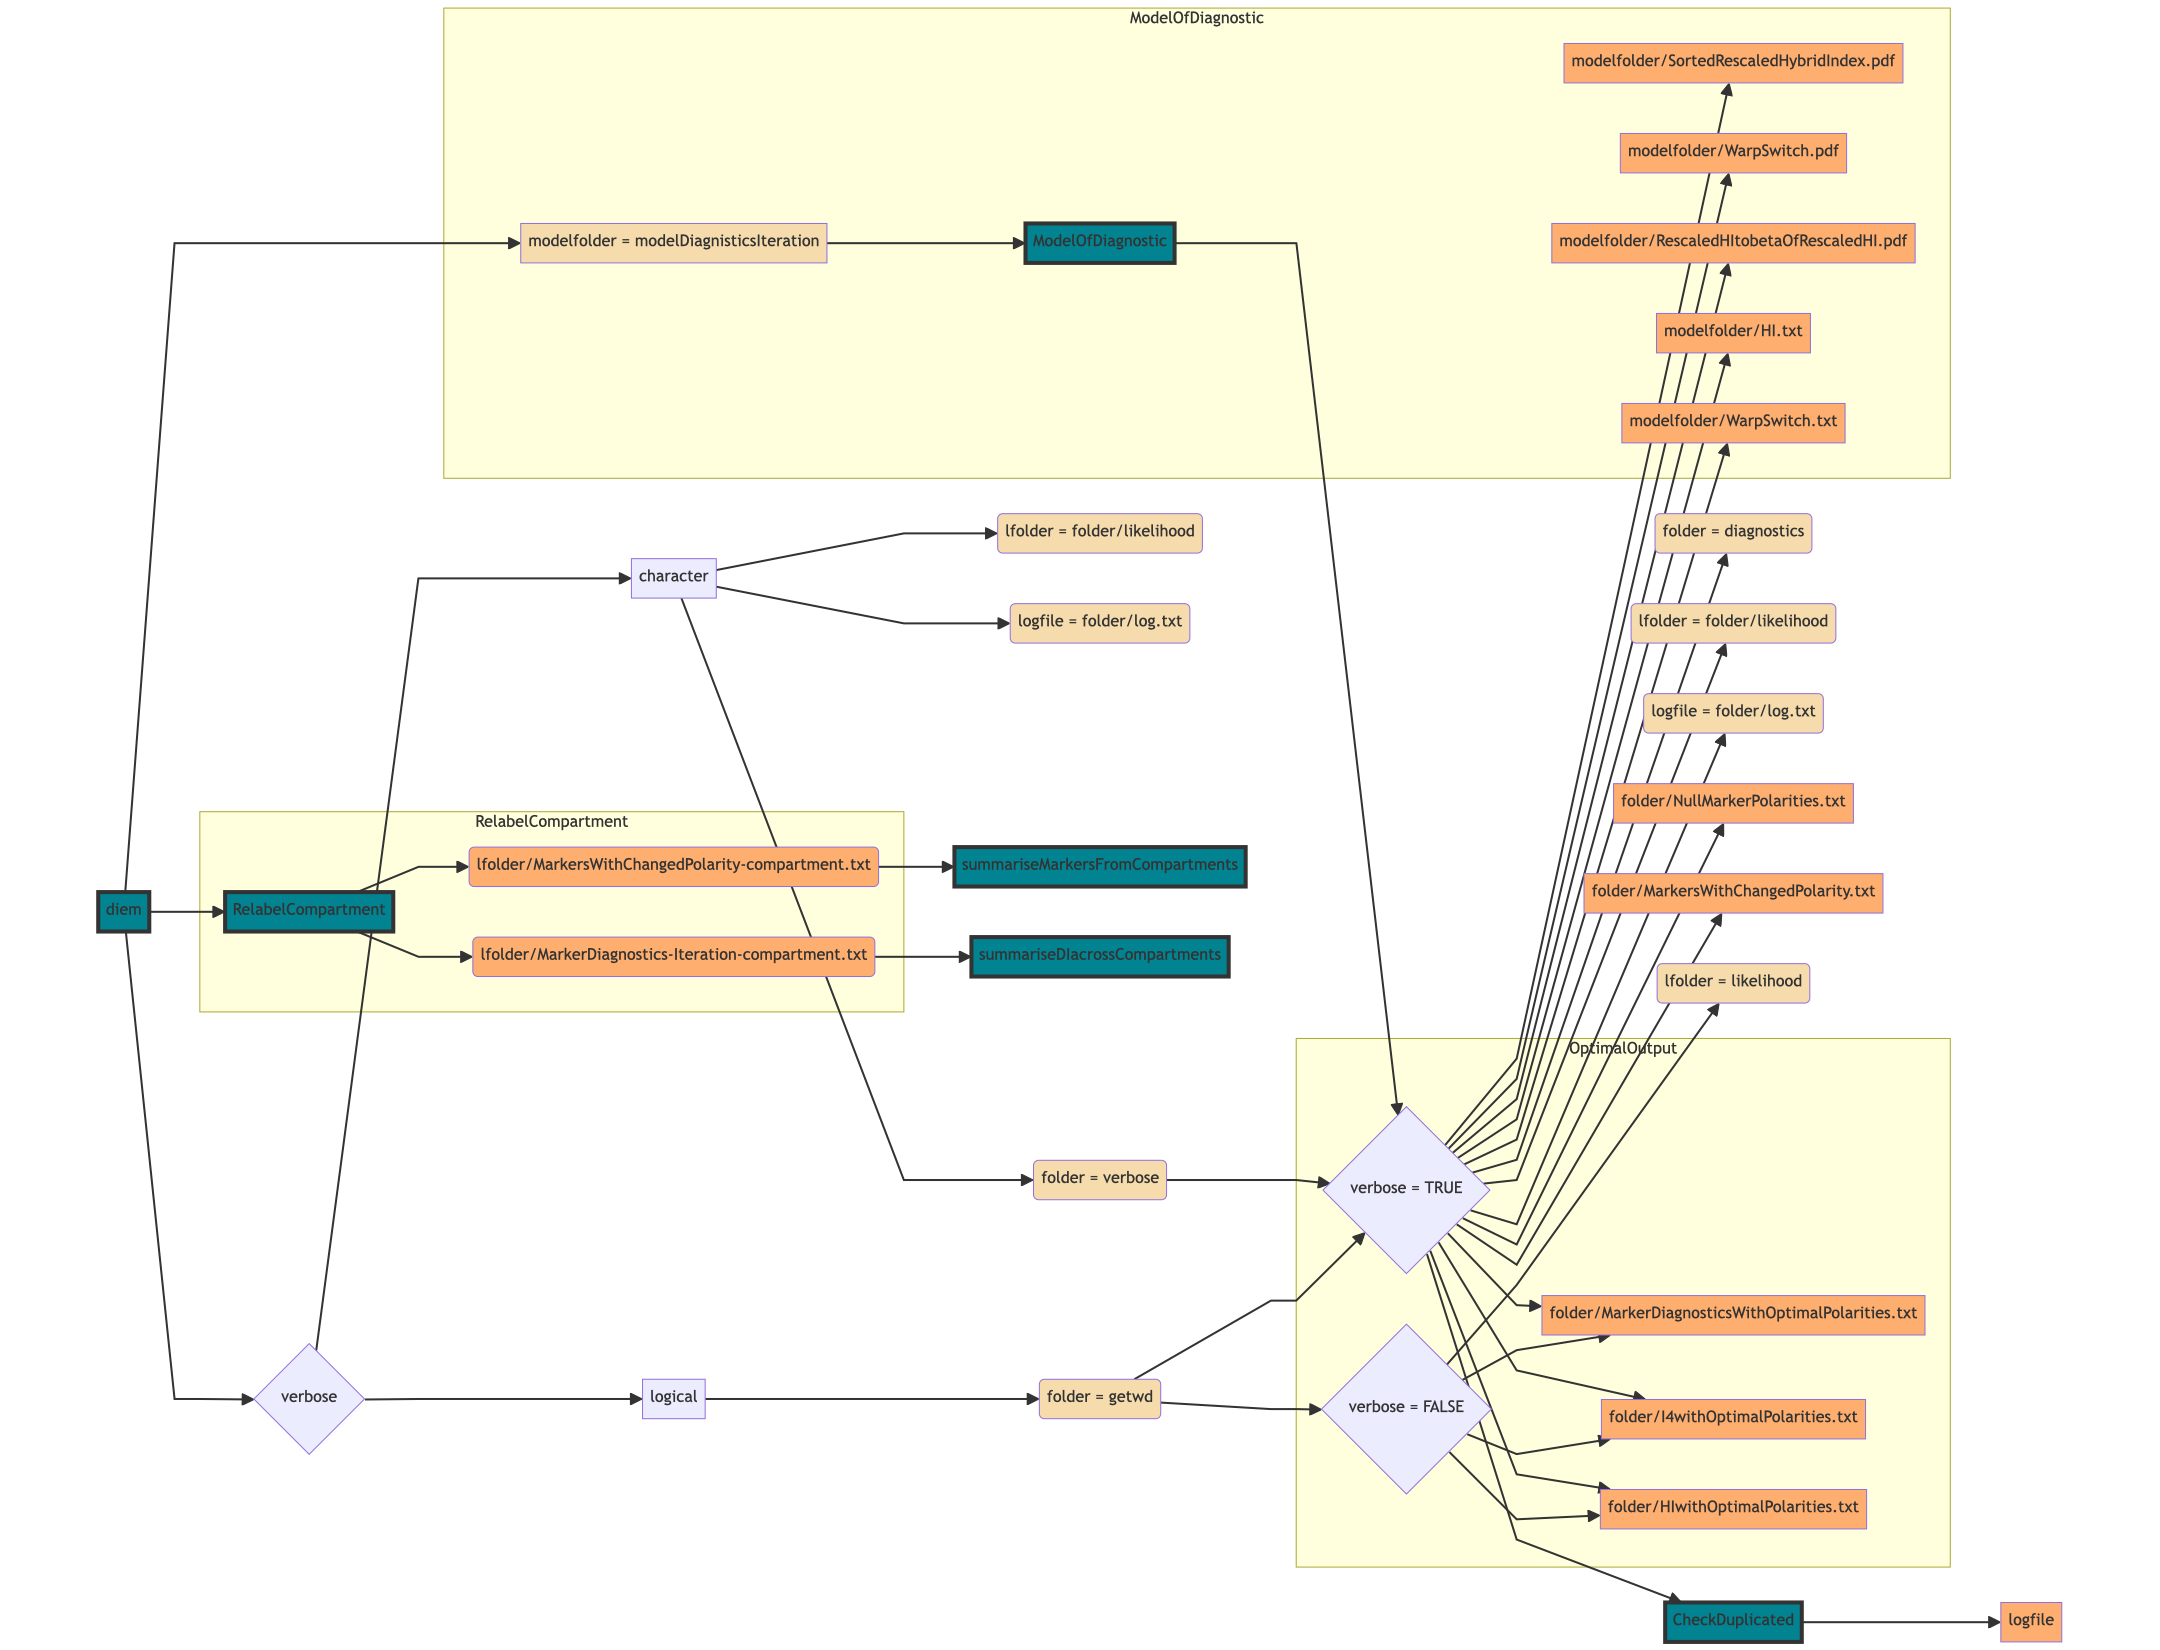
\includegraphics[width=1\linewidth]{figs/diemOutput} 

}

\caption{**Figure 1**. Flowchart of how to control output files and their location in `diem`. Green -- functions generating or using the files. Except `diem` all functions are internal. Beige, grey -- variable values set by the user (grey) or by internal processes (beige). Orange -- stored output files. Yellow rectangles -- main processes generating files.}\label{fig:unnamed-chunk-1}
\end{figure}

\subsection{The user perspective}\label{the-user-perspective}

The \texttt{verbose} argument in the \texttt{diem} function controls the stored output files. The default value \texttt{verbose\ =\ FALSE} writes three \hyperref[defaults]{key output files} in the current working directory (\hyperref[fig1]{Figure 1}). To locate the files, the current working directory can be found with:

\begin{Shaded}
\begin{Highlighting}[]
\FunctionTok{getwd}\NormalTok{()}
\end{Highlighting}
\end{Shaded}

Additionally, the \texttt{verbose} argument can trigger a verbose output in two ways.

\begin{enumerate}
\def\labelenumi{\arabic{enumi}.}
\tightlist
\item
  When \texttt{verbose} contains a character string with a path to a specific folder, the verbose output will be stored in that location.
\item
  When \texttt{verbose\ =\ TRUE}, the verbose output will be stored in the current working directory.
\end{enumerate}

\subsection{NullMarkerPolarities}\label{nullmarkerpolarities}

The optimal approach to genome polarisation with \texttt{diem} is to strip all possible data cues before the analysis. In this way, if \texttt{diem} finds a barrier you can be certain it is an intrinsic property of the data. Using random initial marker polarities is central to this approach. We recommend setting the \texttt{diem} argument \texttt{markerPolarity\ =\ FALSE}. The function then generates random polarities for the initiation of the algorithm iterations.

This initial state for \texttt{diem} is saved in file \emph{NullMarkerPolarities.txt}. It is a text file the first line describing the contents of the file. The following lines show space-separated TRUE or FALSE values, where each row corresponds to a compartment as they were specified in the \texttt{files} argument in \texttt{diem}. Because \texttt{diem} is a deterministic algorithm, if you start it from the same initial state, you will get precisely the same answer. You can test this by setting \texttt{markerPolarity} to be the list from \emph{NullMarkerPolarities}.

\begin{Shaded}
\begin{Highlighting}[]
\NormalTok{nullPolarities }\OtherTok{\textless{}{-}} \FunctionTok{readLines}\NormalTok{(}\StringTok{"folder/NullMarkerPolarities.txt"}\NormalTok{)[}\SpecialCharTok{{-}}\DecValTok{1}\NormalTok{]}
\NormalTok{nullPolarities }\OtherTok{\textless{}{-}} \FunctionTok{lapply}\NormalTok{(}
    \FunctionTok{strsplit}\NormalTok{(nullPolarities, }\AttributeTok{split =} \StringTok{" "}\NormalTok{),}
\NormalTok{    as.logical}
\NormalTok{)}
\FunctionTok{diem}\NormalTok{(..., }\AttributeTok{markerPolarities =}\NormalTok{ nullPolarities)}
\end{Highlighting}
\end{Shaded}

You can also test the convergence of the algorithm from different initial states by running the same analysis, but each time generating a new random null by setting \texttt{markerPolarities\ =\ FALSE}.

\subsection{MarkersWithChangedPolarities}\label{changedPolarities}

The file \emph{MarkersWithChangedPolarities.txt} is a tab-delimited file with three columns and a variable number of rows. The column \textbf{changedMarkers} shows indices of markers across all compartments for which the polarity was changed in the given iteration compared to the marker polarity in the previous iteration. The column \textbf{time} gives a time stamp of when the changes were recorded. The column \textbf{iteration} specifies the iteration of the algorithm.

Note that here, markers are pooled across all compartments. The information is useful in tracking convergence in postprocessing, and so is not of interest to the casual user. During the analysis run, keeping the information about polarity changes separate for each compartment is computationally more tractable, especially in parallel processing. A set of files specifying the information for each compartment is stored in a \emph{likelihood} folder (\hyperref[fig1]{Figure 1}).

\subsubsection{MarkersWithChangedPolarities-(compartmentNumber)}\label{markerswithchangedpolarities-compartmentnumber}

The contents of the files is analogical as in the \hyperref[changedPolarities]{\emph{MarkersWithChangedPolarities.txt}}. The difference being that the marker indices are sequential for each compartment.

\subsubsection{MarkerDiagnostics(iteration)-(compartmentNumber)}\label{markerdiagnosticsiteration-compartmentnumber}

The contents of the files correspond to the contents of the \hyperref[markerDiagnostics]{\emph{MarkerDiagnosticsWithOptimalPolarities.txt}}. Here, the polarities, diagnostic indices and their supports are reported separately for each iteration and for each compartment.

Both sets of compartment-specific temporary files are initially stored regardless of the value in the \texttt{verbose} argument, as they are used internally during the analysis. When \texttt{verbose\ =\ FALSE}, \texttt{diem} attempts to delete the \emph{likelihood} folder on exit.

\subsection{Iteration-specific graphics}\label{iteration-specific-graphics}

The internal \texttt{ModelOfDiagnostic} function implements Eq. 19 \citep{Baird2023} that is the powerful tool to detect the most prominent barrier to geneflow in the data. Seeing how individuals become separated on either side of the barrier provides insights into the algorithm convergence.

\subsubsection{WarpSwitch files}\label{warpswitch-files}

The \emph{WarpSwitch.pdf} files plot differences in sorted rescaled hybrid indices (Eq. 12) used to identify the barrier to geneflow \citep{Baird2023}. The \emph{WarpSwitch.txt} files then describe what genomic states the ideal diagnostic marker would have for all included individuals (Eq. 13), and how the ideal 4-genomic state count matrix (Eq. 14) would look like for the first ten individuals.

\subsubsection{Hybrid index files}\label{hybrid-index-files}

The \emph{SortedRescaledHybridIndex.pdf} shows how the differences in hybrid indices between individuals belonging to either side of the barrier become more pronounced with progressing iterations. Note that in order to identify which individuals are placed where, one needs to replicate the figure from \hyperref[HI]{hybrid index} values in files \emph{HI.txt}.

The files \emph{RescaledHItobetaOfRescaledHI.pdf} show the weight for the hybrid index (Eq. 15) that together with the parameter value in the \texttt{diem} argument \texttt{epsilon} will inform on how much emphasis the analysis puts on the ideal state with the center of the barrier identified in the WarpSwich files.

The visualisation in the iteration-specific graphics provide a tangible track record of how the theoretical ideals of pure individuals and perfectly diagnostic markers contribute to informing on a barrier to geneflow in a realistic scenario, where there are no pure individuals and no perfectly diagnostic markers.

\subsection{The log file}\label{the-log-file}

The \emph{log.txt} file provides a human-readable overview of the \texttt{diem} iterations. During initialisation stage, the log file will list the number of markers and individuals in the analysis run, followed by the top seven rows of the \hyperref[I4]{4-genomic state count matrix \({}^4\mathbf{I}\)} with null polarisation, correction for small data (Eq. 5), top seven rows of the \({}^4\mathbf{A}\), which is the \({}^4\mathbf{I}\) matrix corrected for compartment- and individual-specific ploidies and is used to calculate the hybrid index, the top seven rows of the weighted \({}^4\mathbf{V}\) matrix (Eq. 16), and the respective log-likelihood values (Eq. 19).

For subsequent iterations, the log file also quantifies how many markers switch polarities between iterations, and shows the corresponding change to the \({}^4\mathbf{I}\).

\chapter{Visualisation of polarised genotypes}\label{visualisation-of-polarised-genotypes}

Visualisation is a key step in interpreting the results of genome polarisation.
The \texttt{diemr} package provides several functions for graphical inspection of polarised genotypes, including \texttt{plotPolarized} for genome-wide patterns, \texttt{plotMarkerAxis} for adding chromosome information, and \texttt{plotDeFinetti} for individual genotype composition summaries.

\section{Plotting polarised genotypes}\label{plotting-polarised-genotypes}

The function \texttt{plotPolarized} displays genotypes in either a rectangular or a circular (iris-style) layout.
Rows represent individuals and columns represent single-nucleotide variants (SNVs).
Colours correspond to genotype states: by default, purple and green mark the two homozygote classes (\texttt{0} and \texttt{2}), yellow marks heterozygotes (\texttt{1}), and white indicates missing data (\texttt{\_}).

The polarised genotypes must first be imported with correct site polarity. The polarity will be in memory in element \texttt{res\$markerPolarity} described in (Chapter \ref{intro}) or in the obligatory output file \emph{MarkerDiagnosticsWithOptimalPolarities.txt} (Chapter \ref{markerDiagnostics}) in the column \texttt{newPolarity}.

\begin{Shaded}
\begin{Highlighting}[]
\CommentTok{\# Import polarised genotypes}
\NormalTok{gen }\OtherTok{\textless{}{-}} \FunctionTok{importPolarized}\NormalTok{(}
  \AttributeTok{file =} \FunctionTok{system.file}\NormalTok{(}\StringTok{"extdata"}\NormalTok{, }\StringTok{"data7x10.txt"}\NormalTok{, }\AttributeTok{package =} \StringTok{"diemr"}\NormalTok{),}
  \AttributeTok{changePolarity =} \FunctionTok{c}\NormalTok{(}\ConstantTok{TRUE}\NormalTok{, }\ConstantTok{FALSE}\NormalTok{, }\ConstantTok{TRUE}\NormalTok{, }\ConstantTok{TRUE}\NormalTok{, }\ConstantTok{FALSE}\NormalTok{, }\ConstantTok{FALSE}\NormalTok{, }\ConstantTok{TRUE}\NormalTok{, }\ConstantTok{FALSE}\NormalTok{, }\ConstantTok{FALSE}\NormalTok{, }\ConstantTok{TRUE}\NormalTok{),}
  \AttributeTok{ChosenInds =} \DecValTok{1}\SpecialCharTok{:}\DecValTok{7}
\NormalTok{)}

\CommentTok{\# Calculate individual hybrid indices from the imported genotypes }
\NormalTok{HI }\OtherTok{\textless{}{-}} \FunctionTok{hybridIndex}\NormalTok{(gen)}
\end{Highlighting}
\end{Shaded}

\subsection{Rectangular plot}\label{rectangular-plot}

The rectangular layout is useful for viewing the order of markers along the genome and for comparing individual hybrid indices along the vertical axis. This is the default plot, and uses the matrix of polarised genotypes and the numeric vector of individual hybrid indices.

\begin{Shaded}
\begin{Highlighting}[]
\FunctionTok{plotPolarized}\NormalTok{(}\AttributeTok{genotypes =}\NormalTok{ gen, }\AttributeTok{HI =}\NormalTok{ HI, }\AttributeTok{useRaster =} \ConstantTok{FALSE}\NormalTok{)}
\end{Highlighting}
\end{Shaded}

\begin{center}
\includegraphics{04-Visualisation_files/figure-latex/unnamed-chunk-3-1} \end{center}

Each individual is plotted in order of increasing hybrid index, from bottom to top.
A colour transition across the plot reveals the genomic gradient between parental sides.

\subsubsection{Adding chromosome information}\label{plotMarkerAxis}

If the input data were generated from a VCF file, marker positions are already available.
The file \texttt{*-includedSites.txt} produced by \texttt{vcf2diem} stores physical coordinates for each marker and can be used to draw chromosome names and position ticks beneath the genotype matrix. This file links plotted markers to their genomic locations.

The following example uses a snippet of SNV data with \emph{Myotis} bat diversity \citep{Harazim2021}.

\begin{Shaded}
\begin{Highlighting}[]
\CommentTok{\# Prepare input data}
\NormalTok{myo }\OtherTok{\textless{}{-}} \FunctionTok{system.file}\NormalTok{(}\StringTok{"extdata"}\NormalTok{, }\StringTok{"myotis.vcf"}\NormalTok{, }\AttributeTok{package =} \StringTok{"diemr"}\NormalTok{)}
\FunctionTok{vcf2diem}\NormalTok{(}\AttributeTok{SNP =}\NormalTok{ myo, }\AttributeTok{filename =} \StringTok{"myo"}\NormalTok{)}
\NormalTok{inds }\OtherTok{\textless{}{-}} \DecValTok{1}\SpecialCharTok{:}\DecValTok{14}


\CommentTok{\# Polarise genotypes assuming diploid data}
\NormalTok{res }\OtherTok{\textless{}{-}} \FunctionTok{diem}\NormalTok{(}\StringTok{"myo{-}001.txt"}\NormalTok{, }\AttributeTok{ChosenInds =}\NormalTok{ inds, }\AttributeTok{ploidy =} \ConstantTok{FALSE}\NormalTok{)}

\CommentTok{\# Import polarised genotypes}
\NormalTok{gen }\OtherTok{\textless{}{-}} \FunctionTok{importPolarized}\NormalTok{(}\StringTok{"myo{-}001.txt"}\NormalTok{, }
    \AttributeTok{changePolarity =}\NormalTok{ res}\SpecialCharTok{$}\NormalTok{markerPolarity, }
    \AttributeTok{ChosenInds =}\NormalTok{ inds)}
    
\CommentTok{\# Calculate hybrid indices  }
\NormalTok{HI }\OtherTok{\textless{}{-}} \FunctionTok{hybridIndex}\NormalTok{(gen)}

\CommentTok{\# Plot polarised genotypes with the marker axis }
\FunctionTok{plotPolarized}\NormalTok{(}
  \AttributeTok{genotypes =}\NormalTok{ gen,}
  \AttributeTok{HI =}\NormalTok{ HI,}
  \AttributeTok{addMarkerAxis =} \ConstantTok{TRUE}\NormalTok{,}
  \AttributeTok{includedSites =} \StringTok{"myo{-}includedSites.txt"}\NormalTok{,}
  \AttributeTok{tickDist =} \DecValTok{100}
\NormalTok{)}
\end{Highlighting}
\end{Shaded}

\begin{center}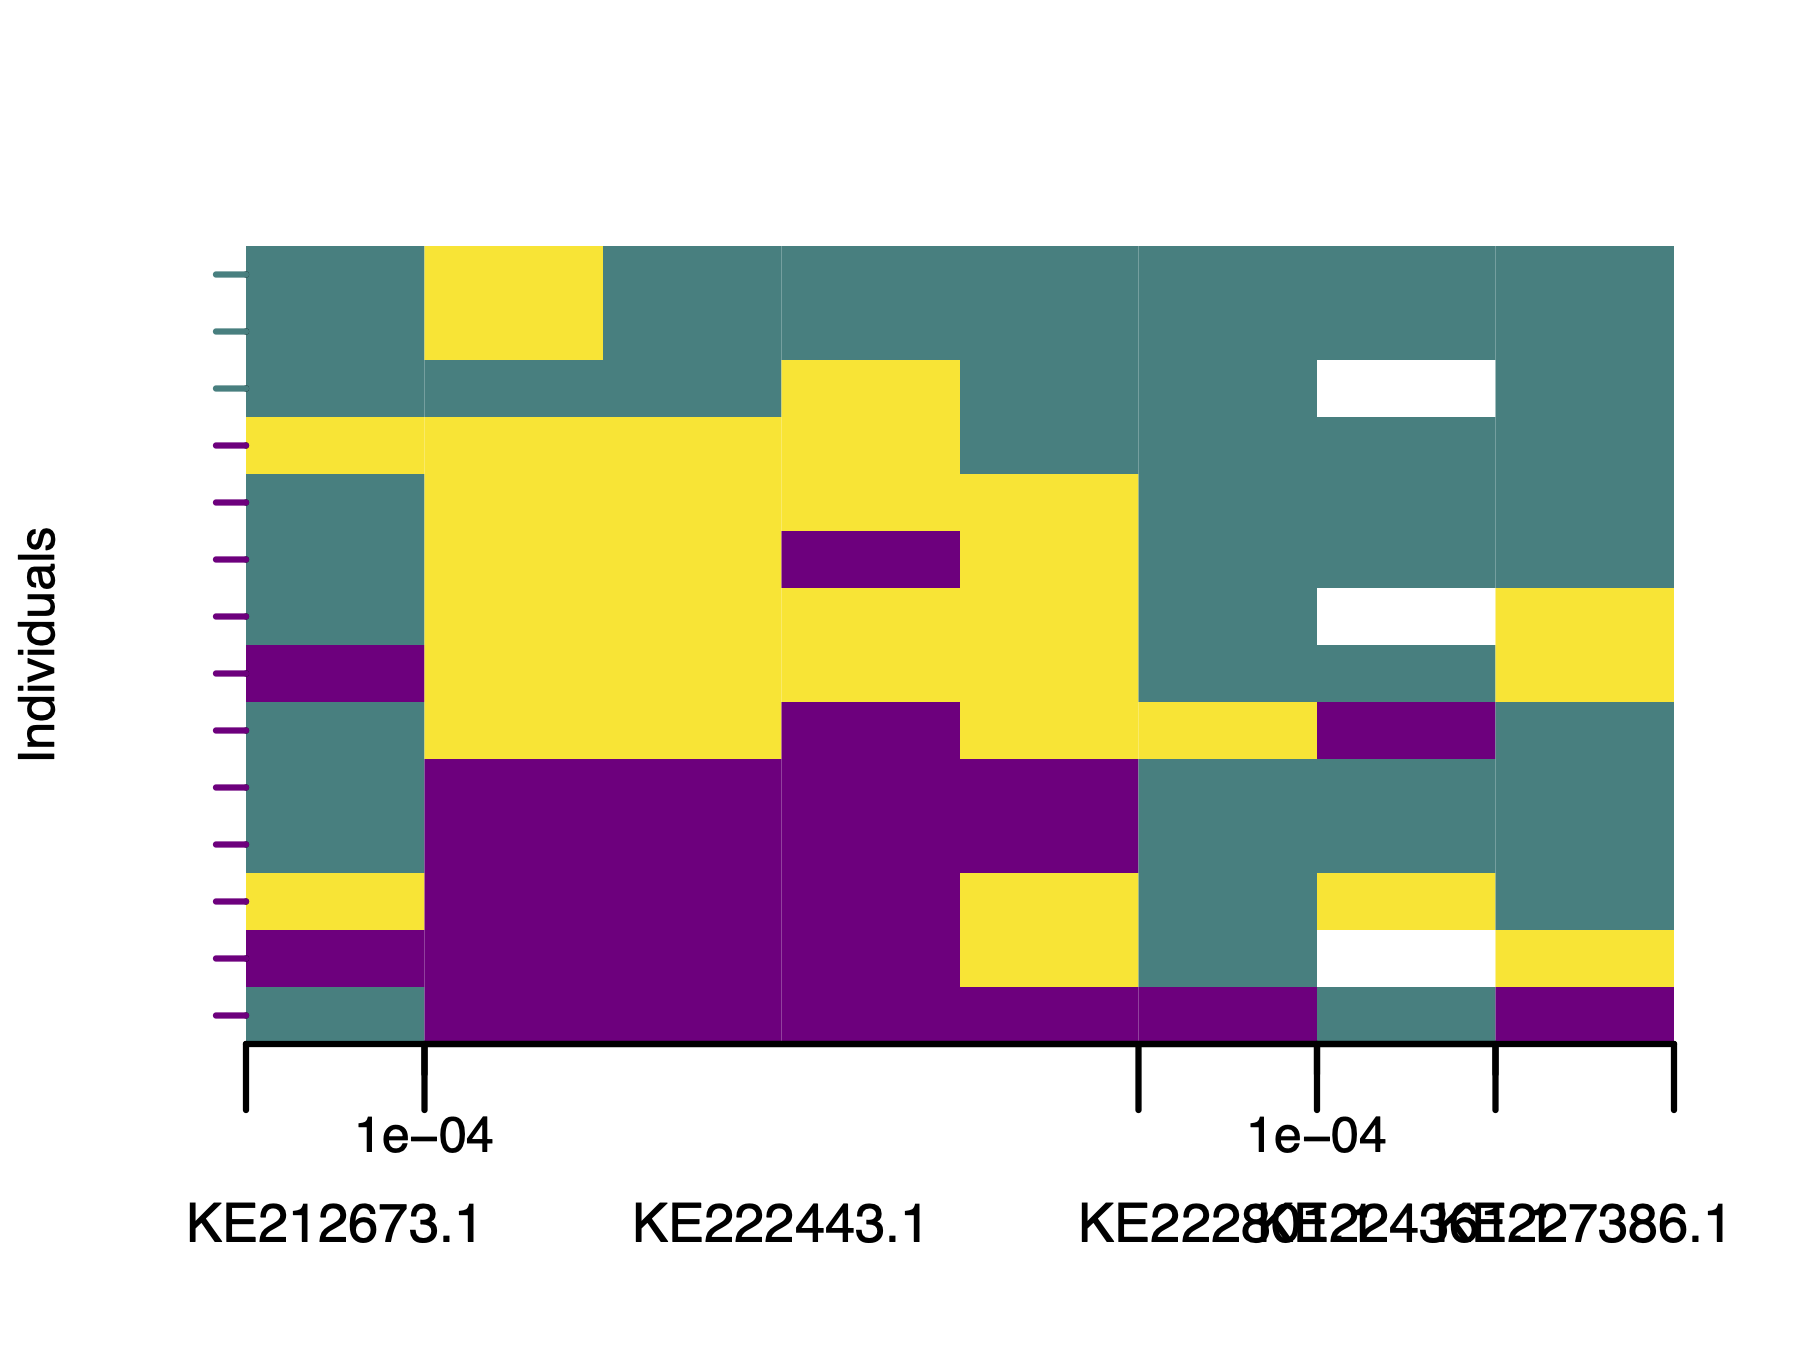
\includegraphics[width=1\linewidth]{figs/myo-rectangle} \end{center}

If the default marker axis needs adjustments, such as here, where accession numbers overlap, use \texttt{plotMarkerAxis} directly. This returns an \texttt{axisInfo} list so you can modify labels before redrawing. \texttt{plotMarkerAxis} also accepts additional graphical arguments.

\begin{Shaded}
\begin{Highlighting}[]
\CommentTok{\# Draw plot without axis}
\FunctionTok{plotPolarized}\NormalTok{(}
  \AttributeTok{genotypes =}\NormalTok{ gen,}
  \AttributeTok{HI =}\NormalTok{ HI,}
  \AttributeTok{addMarkerAxis =} \ConstantTok{FALSE}\NormalTok{,}
  \AttributeTok{xlab =} \StringTok{""}
\NormalTok{)}

\CommentTok{\# Draw marker axis, and capture axis information}
\NormalTok{axisInfo }\OtherTok{\textless{}{-}} \FunctionTok{plotMarkerAxis}\NormalTok{(}\AttributeTok{includedSites =} \StringTok{"myo{-}includedSites.txt"}\NormalTok{, }\AttributeTok{tickDist =} \DecValTok{100}\NormalTok{)}
\end{Highlighting}
\end{Shaded}

The \texttt{axisInfo} list will now contain five elements with plotting data. Let's shorten the contig names and convert the tick labels to base pairs (default is to display milions of base pairs). This list can then be used for plotting directly, without the need to recalculate the position of the axis elements from the \texttt{*-includedSites.txt} file.

\begin{Shaded}
\begin{Highlighting}[]
\FunctionTok{print}\NormalTok{(axisInfo)}
\CommentTok{\# $CHROMbreaks}
\CommentTok{\# [1] 0.5 1.5 5.5 6.5 7.5 8.5}
\CommentTok{\# }
\CommentTok{\# $CHROMnamesPos}
\CommentTok{\# [1] 1.0 3.5 6.0 7.0 8.0}
\CommentTok{\# }
\CommentTok{\# $CHROMnames}
\CommentTok{\# [1] "KE212673.1" "KE222443.1" "KE222801.1" "KE224361.1" "KE227386.1"}
\CommentTok{\# }
\CommentTok{\# $ticksPos}
\CommentTok{\# [1] 1.5 6.5 7.5}
\CommentTok{\# }
\CommentTok{\# $ticksNames}
\CommentTok{\# [1] 1e{-}04 1e{-}04 1e{-}04}

\CommentTok{\# Update list elements}
\NormalTok{axisInfo}\SpecialCharTok{$}\NormalTok{CHROMnames }\OtherTok{\textless{}{-}} \FunctionTok{c}\NormalTok{(}\StringTok{"con1"}\NormalTok{, }\StringTok{"con2"}\NormalTok{, }\StringTok{"con3"}\NormalTok{, }\StringTok{"con4"}\NormalTok{, }\StringTok{"con5"}\NormalTok{)}
\NormalTok{axisInfo}\SpecialCharTok{$}\NormalTok{ticksNames }\OtherTok{\textless{}{-}} \FunctionTok{c}\NormalTok{(}\DecValTok{100}\NormalTok{, }\DecValTok{100}\NormalTok{, }\DecValTok{100}\NormalTok{)}

\CommentTok{\# Plot polarised genotypes with updated marker axis labels}
\FunctionTok{plotPolarized}\NormalTok{(}
  \AttributeTok{genotypes =}\NormalTok{ gen,}
  \AttributeTok{HI =}\NormalTok{ HI,}
  \AttributeTok{addMarkerAxis =} \ConstantTok{FALSE}\NormalTok{,}
  \AttributeTok{xlab =} \StringTok{""}
\NormalTok{)}
\FunctionTok{plotMarkerAxis}\NormalTok{(}\AttributeTok{axisInfo =}\NormalTok{ axisInfo)}
\end{Highlighting}
\end{Shaded}

\begin{center}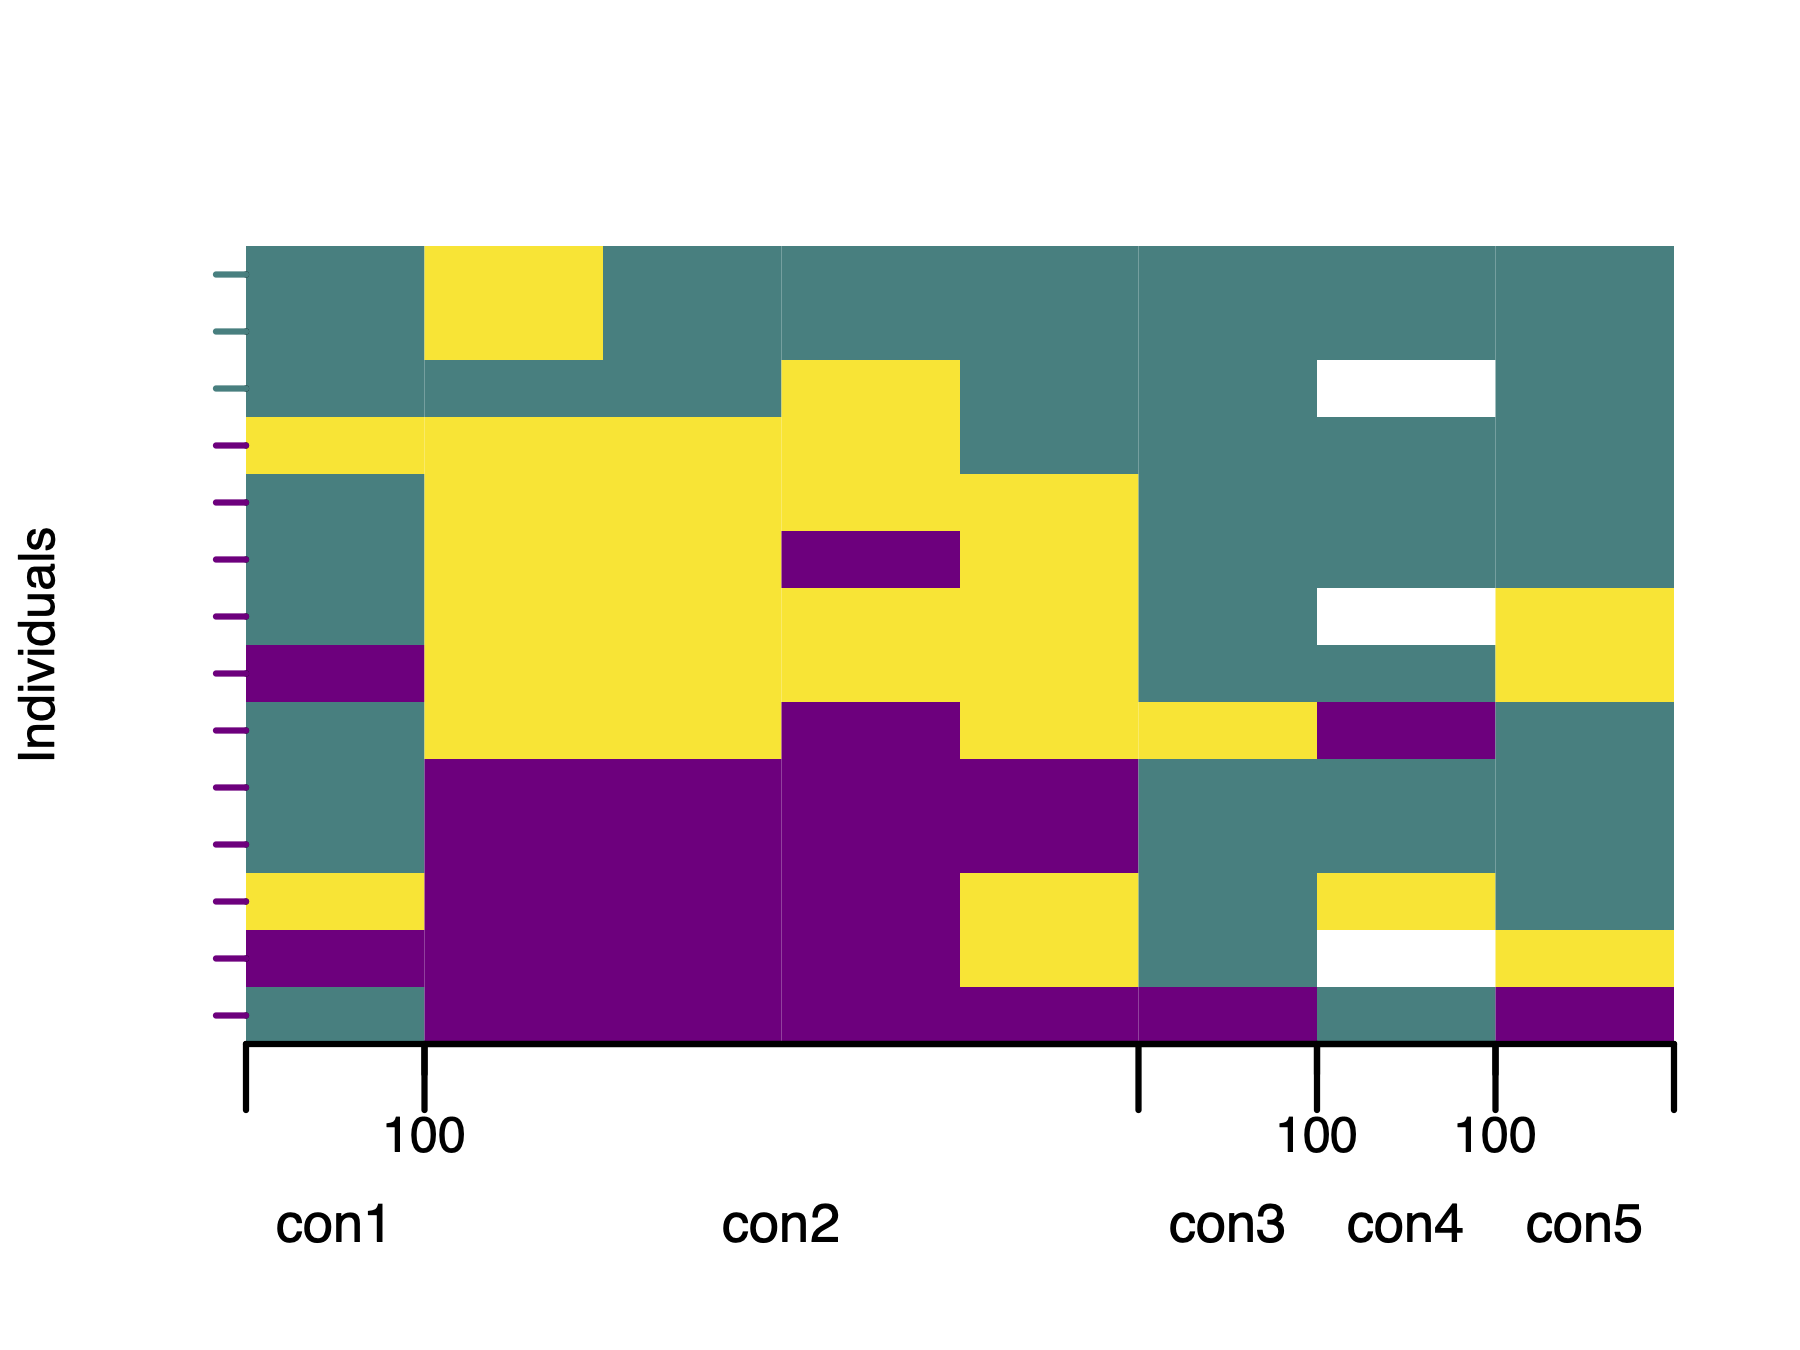
\includegraphics[width=1\linewidth]{figs/myo-rectangle2} \end{center}

\section{Circular (iris) plot}\label{circular-iris-plot}

The circular layout displays the same information radially, emphasising the continuity of ancestry along chromosomes. Individuals are ordered from the centre (lowest hybrid index) to the periphery (highest).

\begin{Shaded}
\begin{Highlighting}[]
\FunctionTok{plotPolarized}\NormalTok{(}\AttributeTok{genotypes =}\NormalTok{ gen, }\AttributeTok{HI =}\NormalTok{ HI, }\AttributeTok{type =} \StringTok{"circular"}\NormalTok{)}
\FunctionTok{plotMarkerAxis}\NormalTok{(}\AttributeTok{axisInfo =}\NormalTok{ axisInfo, }
  \AttributeTok{labels.facing =} \StringTok{"in"}\NormalTok{, }
  \AttributeTok{major.tick.length =} \DecValTok{1}
\NormalTok{)}
\end{Highlighting}
\end{Shaded}


\includegraphics{04-Visualisation_files/figure-latex/unnamed-chunk-10-1.pdf}

The marker axis in circular plots is drawn analogically to rectangular plots (Chapter \ref{plotMarkerAxis}), but chromosome names and tick marks are shown as separate elements. Chromosome names appear in an inner track with alternating white and grey shading, while tick marks showing distances along each chromosome are plotted on the outer rim of the genotype rings.

This layout is compact for displaying genomes of many individuals and highlights symmetry or asymmetry between parental contributions. However, circular plotting of large datasets (more than \(10^5\) markers) can be slow. To monitor progress, set \texttt{showProgress\ =\ TRUE} in \texttt{plotPolarized}. This prints the percentage of plotted individuals to the standard output during rendering.

\chapter{Filtering sites by diagnostic index}\label{DIfiltering}

After obtaining polarised genotypes and diagnostic indices from previous steps, the next step is to identify markers that most clearly distinguish the two sides of the barrier. This chapter demonstrates how to use the diagnostic index (DI) for that purpose. A note in the Chapter \ref{intro} cautioned against using whole-genome summaries for downstream analyses. This chapter expands the \emph{Quick start} introduction.

During genome polarisation, each site receives a likelihood-based \textbf{diagnostic index (DI)} that quantifies its contribution to distinguishing the two sides of the barrier. Sites with low DI are weakly informative and act as noise; they inflate apparent heterogeneity and reduce clarity in hybrid index (HI) plots. Filtering sites by DI allows extraction of informative genomic markers that:

\begin{itemize}
\tightlist
\item
  reduce noise from standing genetic variation,
\item
  produce steeper clines in HI profiles,
\item
  enhance contrast between groups in genotype heatmaps,
\item
  stabilise window‑based summaries.
\end{itemize}

However, filtering is a trade‑off. Retaining too few sites can oversimplify the genomic pattern, while keeping all markers may obscure structure within background noise. No universal DI threshold exists; the optimal cutoff depends on genetic variation within the dataset and the divergence captured by the barrier to gene flow. Therefore, inspect the results visually to decide.

The DI values are exported for all sites, and are either available in the standard output from \texttt{diem} in an element \texttt{DI} in column \texttt{DI} or in the output file \emph{MarkerDiagnosticsWithOptimalPolarities.txt} (Chapter \ref{markerDiagnostics}). This example will demonstrate DI-filtering from the file. Let's first display polarised genotypes without filtering sites by their diagnostic index.

Full code to prepare data to execute the examples in this chapter

\begin{Shaded}
\begin{Highlighting}[]
\FunctionTok{library}\NormalTok{(diemr)}

\NormalTok{dat }\OtherTok{\textless{}{-}} \FunctionTok{system.file}\NormalTok{(}\StringTok{"extdata"}\NormalTok{, }\StringTok{"testBarrier2.txt"}\NormalTok{, }\AttributeTok{package =} \StringTok{"diemr"}\NormalTok{)}
\NormalTok{inds }\OtherTok{\textless{}{-}} \DecValTok{1}\SpecialCharTok{:}\DecValTok{6}

\NormalTok{res }\OtherTok{\textless{}{-}} \FunctionTok{diem}\NormalTok{(}\AttributeTok{files =}\NormalTok{ dat, }\AttributeTok{ChosenInds =}\NormalTok{ inds)}
\end{Highlighting}
\end{Shaded}

\begin{Shaded}
\begin{Highlighting}[]
\CommentTok{\# import polarised genotypes for the diagnostic markers}
\NormalTok{gen }\OtherTok{\textless{}{-}} \FunctionTok{importPolarized}\NormalTok{(}
  \FunctionTok{system.file}\NormalTok{(}\StringTok{"extdata"}\NormalTok{, }\StringTok{"testBarrier2.txt"}\NormalTok{, }\AttributeTok{package =} \StringTok{"diemr"}\NormalTok{),}
  \AttributeTok{changePolarity =}\NormalTok{ DI}\SpecialCharTok{$}\NormalTok{newPolarity,}
  \AttributeTok{ChosenInds =} \DecValTok{1}\SpecialCharTok{:}\DecValTok{6}\NormalTok{,}
  \AttributeTok{ChosenSites =} \StringTok{"all"}
\NormalTok{)}

\CommentTok{\# calculate hybrid indices from the filtered genotypes}
\NormalTok{HI }\OtherTok{\textless{}{-}} \FunctionTok{hybridIndex}\NormalTok{(gen, }\AttributeTok{rescale =} \ConstantTok{TRUE}\NormalTok{)}

\CommentTok{\# plot HI and all genotypes}
\FunctionTok{layout}\NormalTok{(}\FunctionTok{matrix}\NormalTok{(}\FunctionTok{c}\NormalTok{(}\DecValTok{1}\NormalTok{,}\DecValTok{2}\NormalTok{,}\DecValTok{2}\NormalTok{,}\DecValTok{2}\NormalTok{,}\DecValTok{2}\NormalTok{), }\AttributeTok{nrow =} \DecValTok{1}\NormalTok{))}
\NormalTok{indOrder }\OtherTok{\textless{}{-}} \FunctionTok{order}\NormalTok{(HI)}
\CommentTok{\# plot hybrid indices}
\FunctionTok{plot}\NormalTok{(HI[indOrder], }\DecValTok{1}\SpecialCharTok{:}\FunctionTok{length}\NormalTok{(HI), }
  \AttributeTok{xlab =} \StringTok{"Hybrid index"}\NormalTok{, }\AttributeTok{ylab =} \StringTok{"Individuals"}\NormalTok{, }\AttributeTok{axes =} \ConstantTok{FALSE}\NormalTok{,}
  \AttributeTok{ylim =} \FunctionTok{c}\NormalTok{(}\FloatTok{0.5}\NormalTok{, }\FunctionTok{length}\NormalTok{(HI) }\SpecialCharTok{+} \FloatTok{0.5}\NormalTok{), }\AttributeTok{pch =} \DecValTok{19}\NormalTok{,}
  \AttributeTok{yaxs =} \StringTok{"i"}\NormalTok{, }\AttributeTok{xpd =} \ConstantTok{NA}\NormalTok{)}
\CommentTok{\# add axes with ordered individual labels}
\FunctionTok{axis}\NormalTok{(}\DecValTok{1}\NormalTok{)}
\FunctionTok{axis}\NormalTok{(}\DecValTok{2}\NormalTok{, }\AttributeTok{at =} \DecValTok{1}\SpecialCharTok{:}\FunctionTok{length}\NormalTok{(HI), }\AttributeTok{labels =}\NormalTok{ inds[indOrder], }\AttributeTok{las =} \DecValTok{1}\NormalTok{)}
\FunctionTok{box}\NormalTok{()}
\CommentTok{\# plot genotypes}
\FunctionTok{plotPolarized}\NormalTok{(gen, }\AttributeTok{HI =}\NormalTok{ HI, }\AttributeTok{ylab =} \StringTok{""}\NormalTok{)}
\end{Highlighting}
\end{Shaded}

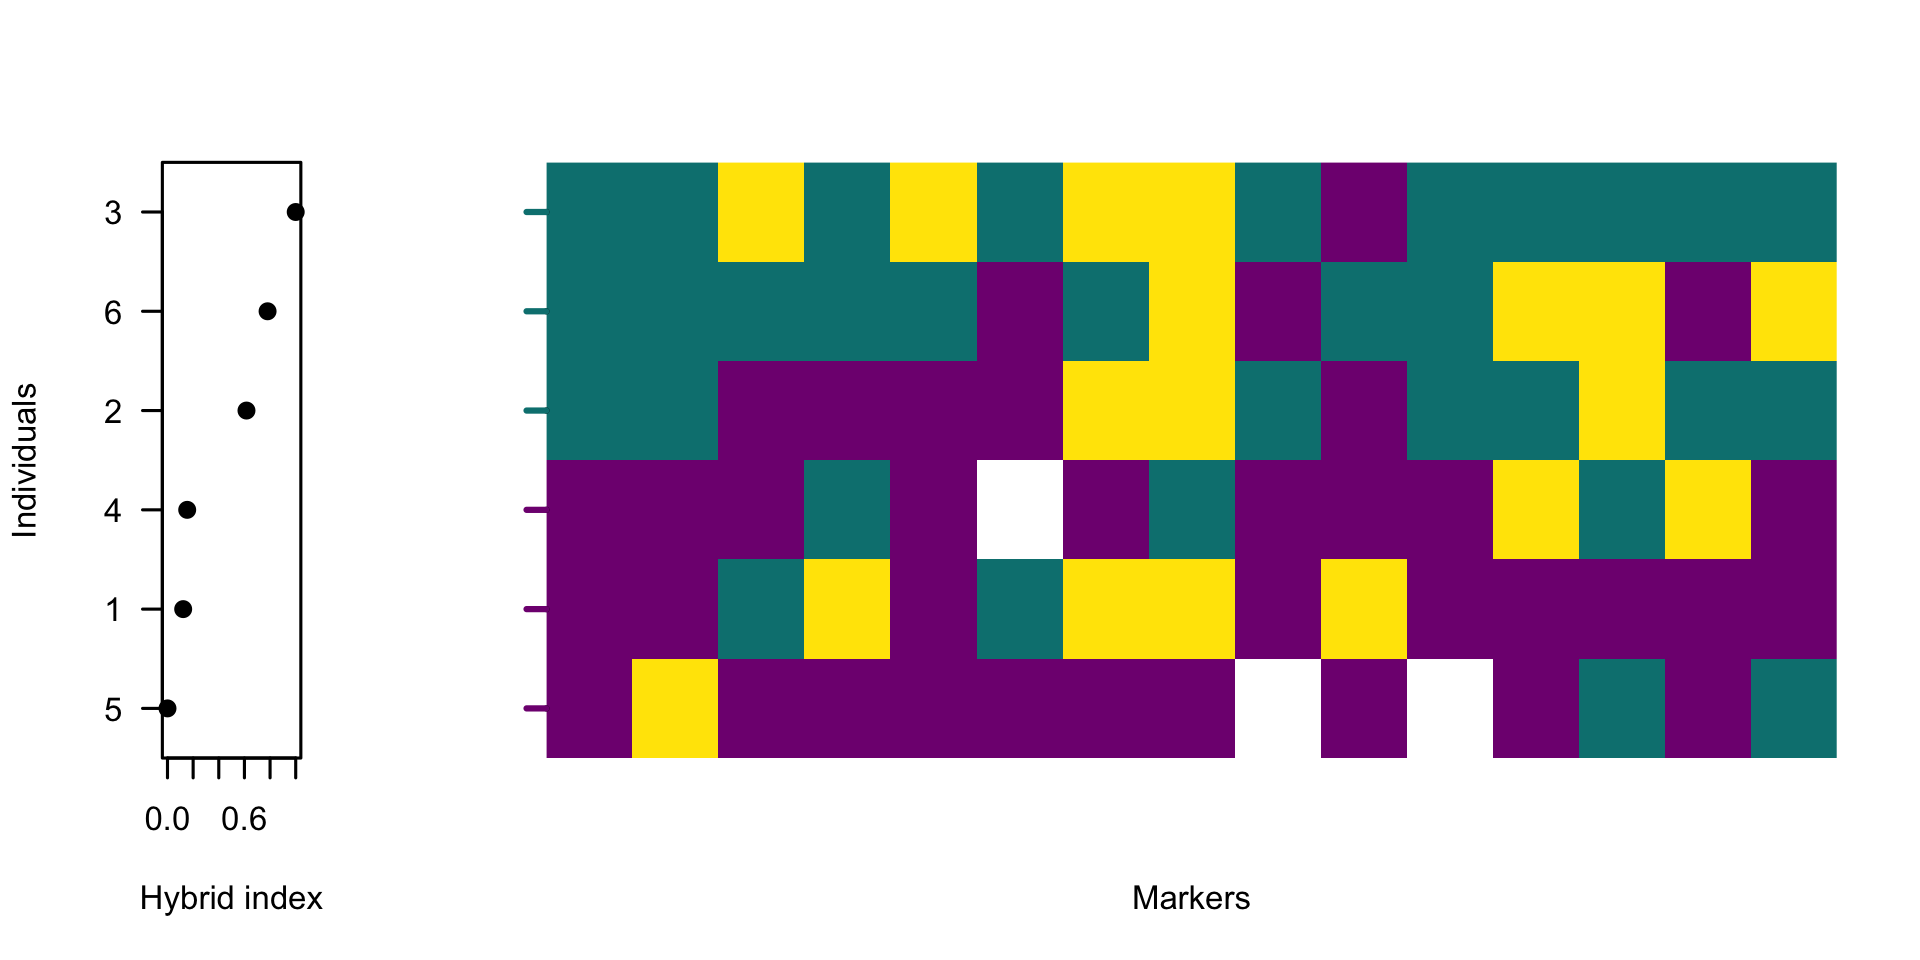
\includegraphics[width=1\linewidth]{figs/testdata-all}

The function \texttt{hybridIndex} estimates the proportion of alleles belonging to one side of the barrier across all polarised sites for each individual, automatically accounting for missing data. \texttt{plotPolarized} orders individuals by their hybrid index. Displaying the hybrid indices alongside a heatmap of polarised genotypes provides a visual guide to the quantitative change in genome admixture.

The figure shows high genetic variability across the data. Next, let's plot only 30\% of markers with the highest diagnostic index.

\begin{Shaded}
\begin{Highlighting}[]
\CommentTok{\# read the marker diagnostics file. read.table is possible, }
\CommentTok{\# but for large genomic datasets, fread is more efficient}
\NormalTok{DI }\OtherTok{\textless{}{-}}\NormalTok{ data.table}\SpecialCharTok{::}\FunctionTok{fread}\NormalTok{(}\StringTok{"MarkerDiagnosticsWithOptimalPolarities.txt"}\NormalTok{, }
  \AttributeTok{header =} \ConstantTok{TRUE}\NormalTok{, }\AttributeTok{data.table =} \ConstantTok{FALSE}
\NormalTok{)}

\CommentTok{\# keep the top 40\% most diagnostic sites}
\NormalTok{threshold }\OtherTok{\textless{}{-}} \FloatTok{0.6}
\NormalTok{whichMarkers }\OtherTok{\textless{}{-}}\NormalTok{ DI}\SpecialCharTok{$}\NormalTok{DI }\SpecialCharTok{\textgreater{}=} \FunctionTok{quantile}\NormalTok{(DI}\SpecialCharTok{$}\NormalTok{DI, }\AttributeTok{probs =}\NormalTok{ threshold)}

\CommentTok{\# calculate hybrid indices from the filtered genotypes}
\NormalTok{HI2 }\OtherTok{\textless{}{-}} \FunctionTok{hybridIndex}\NormalTok{(gen[, whichMarkers], }\AttributeTok{rescale =} \ConstantTok{TRUE}\NormalTok{)}

\CommentTok{\# plot HI and all genotypes}
\FunctionTok{layout}\NormalTok{(}\FunctionTok{matrix}\NormalTok{(}\FunctionTok{c}\NormalTok{(}\DecValTok{1}\NormalTok{,}\DecValTok{2}\NormalTok{,}\DecValTok{2}\NormalTok{,}\DecValTok{2}\NormalTok{,}\DecValTok{2}\NormalTok{), }\AttributeTok{nrow =} \DecValTok{1}\NormalTok{))}
\NormalTok{indOrder2 }\OtherTok{\textless{}{-}} \FunctionTok{order}\NormalTok{(HI2)}
\CommentTok{\# plot hybrid indices}
\FunctionTok{plot}\NormalTok{(HI2[indOrder2], }\DecValTok{1}\SpecialCharTok{:}\FunctionTok{length}\NormalTok{(HI2), }
  \AttributeTok{xlab =} \StringTok{"Hybrid index"}\NormalTok{, }\AttributeTok{ylab =} \StringTok{"Individuals"}\NormalTok{, }\AttributeTok{axes =} \ConstantTok{FALSE}\NormalTok{,}
  \AttributeTok{ylim =} \FunctionTok{c}\NormalTok{(}\FloatTok{0.5}\NormalTok{, }\FunctionTok{length}\NormalTok{(HI) }\SpecialCharTok{+} \FloatTok{0.5}\NormalTok{), }\AttributeTok{pch =} \DecValTok{19}\NormalTok{,}
  \AttributeTok{yaxs =} \StringTok{"i"}\NormalTok{, }\AttributeTok{xpd =} \ConstantTok{NA}\NormalTok{)}
\CommentTok{\# add axes with ordered individual labels}
\FunctionTok{axis}\NormalTok{(}\DecValTok{1}\NormalTok{)}
\FunctionTok{axis}\NormalTok{(}\DecValTok{2}\NormalTok{, }\AttributeTok{at =} \DecValTok{1}\SpecialCharTok{:}\FunctionTok{length}\NormalTok{(HI2), }\AttributeTok{labels =}\NormalTok{ inds[indOrder2], }\AttributeTok{las =} \DecValTok{1}\NormalTok{)}
\FunctionTok{box}\NormalTok{()}
\CommentTok{\# plot genotypes}
\FunctionTok{plotPolarized}\NormalTok{(gen[, whichMarkers], }\AttributeTok{HI =}\NormalTok{ HI2, }\AttributeTok{ylab =} \StringTok{""}\NormalTok{)}
\end{Highlighting}
\end{Shaded}

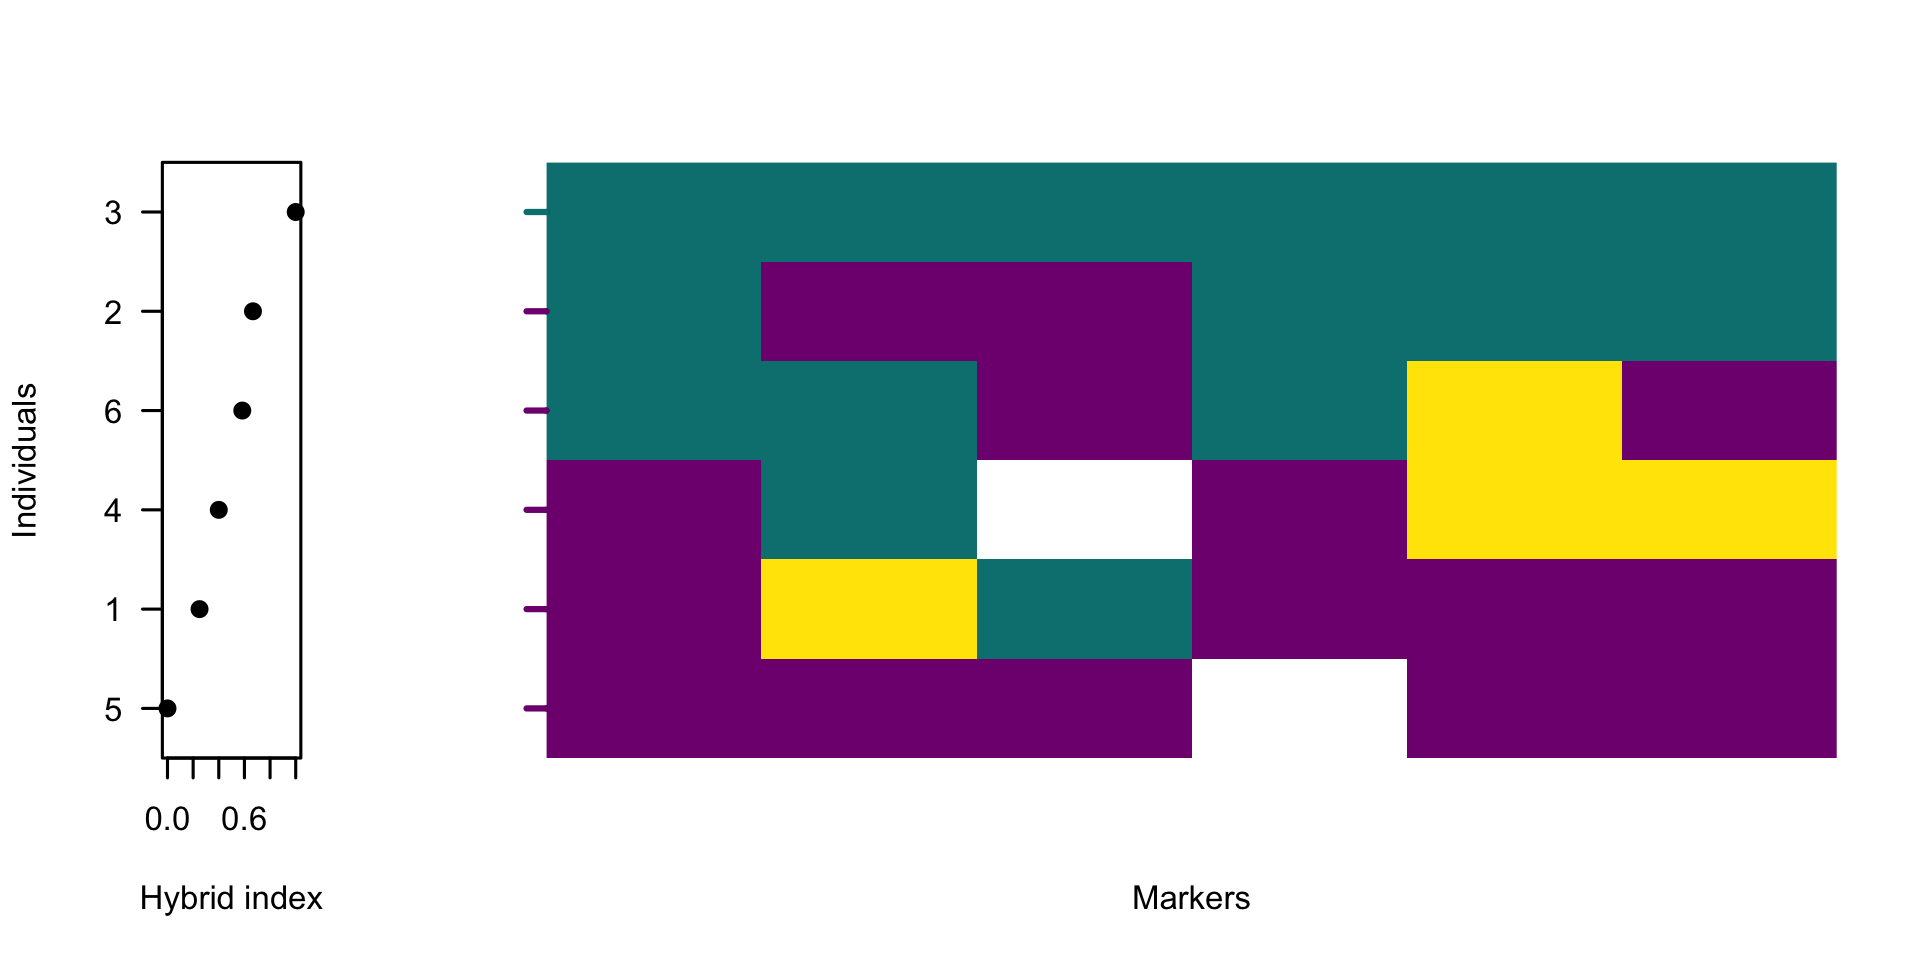
\includegraphics[width=1\linewidth]{figs/testdata-DI40}

\section{Selecting the filtering threshold}\label{selecting-the-filtering-threshold}

With the hybrid index being a proportion of alleles belonging to one side of barrier to gene flow, typical outcome of filtering SNVs by DI is a set of informative markers that shows \textbf{tighter clustering} of individuals near 0 and 1, and a steeper, interpretable gradient across hybrids. However, emphasizing the genomic differences by selecting markers that approach being homozygous on one side of the barrier can have an undesirable effect of highlighting the influence of outliers. These might be inbred individuals, samples with low sequencing coverage or mapping quality or divergent samples informing of a biologically-relevant mechanism. Such individuals are rarely the target of admixture studies, yet they can disproportionately influence the \emph{diem} algorithm and appear as spurious barriers in heavily filtered datasets. To avoid this, the user has two options.

\begin{enumerate}
\def\labelenumi{\arabic{enumi}.}
\tightlist
\item
  To remove the outlier individuals from the analyses using the \texttt{ChosenInds} argument.
\item
  To find the DI filtering threshold that displays the desired barrier to gene flow before it becomes overloaded with outlier pull.
\end{enumerate}

The first option is the cleanest, but both are not mutually exclusive. Let's use the previous example to explore a range of threshold values and their effect on the barrier to gene flow.

\begin{Shaded}
\begin{Highlighting}[]
\NormalTok{thresholds }\OtherTok{\textless{}{-}} \FunctionTok{c}\NormalTok{(}\FloatTok{0.6}\NormalTok{, }\FloatTok{0.7}\NormalTok{, }\FloatTok{0.8}\NormalTok{, }\FloatTok{0.9}\NormalTok{)}

\CommentTok{\# inspect distribution of DI values}
\FunctionTok{hist}\NormalTok{(DI}\SpecialCharTok{$}\NormalTok{DI, }\AttributeTok{xlab =} \StringTok{"Diagnostic index"}\NormalTok{, }\AttributeTok{n =} \DecValTok{20}\NormalTok{, }\AttributeTok{main =} \StringTok{""}\NormalTok{)}
\FunctionTok{abline}\NormalTok{(}\AttributeTok{v =} \FunctionTok{quantile}\NormalTok{(DI}\SpecialCharTok{$}\NormalTok{DI, }\AttributeTok{probs =}\NormalTok{ thresholds), }\AttributeTok{col =} \StringTok{"red"}\NormalTok{, }\AttributeTok{lty =} \DecValTok{2}\NormalTok{)}
\end{Highlighting}
\end{Shaded}

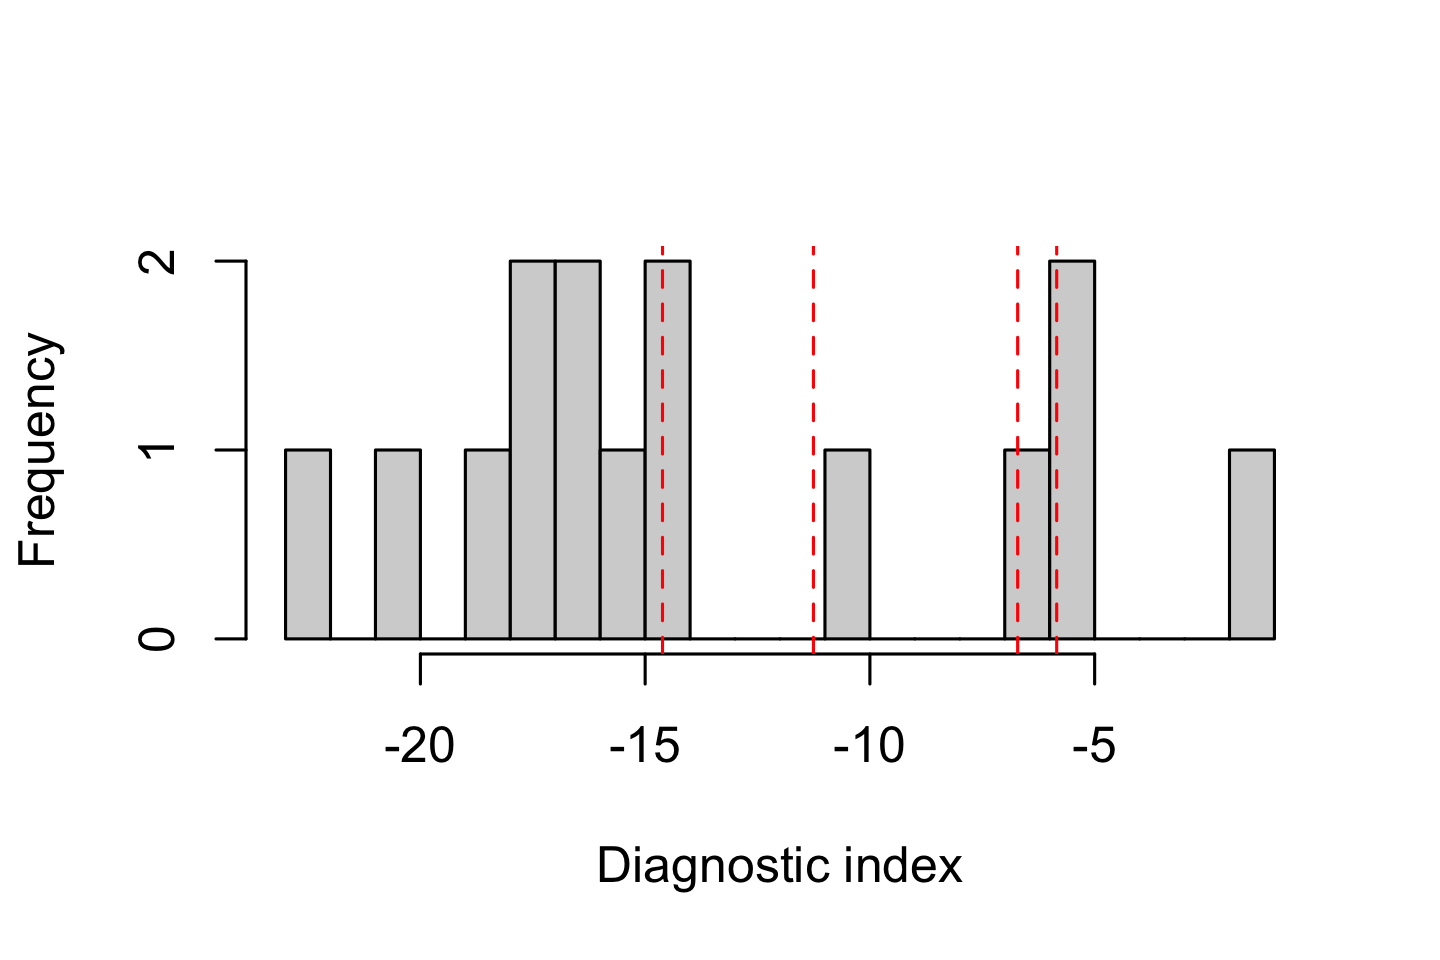
\includegraphics[width=1\linewidth]{figs/hist}

Plotting the DI distribution helps identify whether the dataset has a natural break or continuous spectrum of diagnostic values, guiding selection of a reasonable cutoff. Often in genomic datasets, the distribution of DI values is unimodal. In such cases, exploring how DI filtering affects hybrid index profiles is often a more informative way to select an appropriate threshold.

\begin{Shaded}
\begin{Highlighting}[]
\CommentTok{\# load HI from the ploidy{-}aware whole{-}genome HI in diem output}
\NormalTok{HI }\OtherTok{\textless{}{-}} \FunctionTok{hybridIndex}\NormalTok{(}\StringTok{"HIwithOptimalPolarities.txt"}\NormalTok{, }\AttributeTok{rescale =} \ConstantTok{FALSE}\NormalTok{)}
\NormalTok{indOrder }\OtherTok{\textless{}{-}} \FunctionTok{order}\NormalTok{(HI)}

\FunctionTok{layout}\NormalTok{(}\FunctionTok{matrix}\NormalTok{(}\FunctionTok{c}\NormalTok{(}\DecValTok{1}\NormalTok{,}\DecValTok{1}\NormalTok{,}\DecValTok{1}\NormalTok{,}\DecValTok{2}\NormalTok{), }\AttributeTok{nrow =} \DecValTok{1}\NormalTok{))}
\FunctionTok{plot}\NormalTok{(HI[indOrder], }\AttributeTok{pch =} \DecValTok{19}\NormalTok{, }\AttributeTok{ylim =} \FunctionTok{c}\NormalTok{(}\DecValTok{0}\NormalTok{, }\DecValTok{1}\NormalTok{),}
    \AttributeTok{xlab =} \StringTok{"Individuals"}\NormalTok{, }\AttributeTok{ylab =} \StringTok{"Hybrid index"}
\NormalTok{)}

\ControlFlowTok{for}\NormalTok{ (threshold }\ControlFlowTok{in}\NormalTok{ thresholds)\{}
\NormalTok{  whichMarkers }\OtherTok{\textless{}{-}}\NormalTok{ DI}\SpecialCharTok{$}\NormalTok{DI }\SpecialCharTok{\textgreater{}=} \FunctionTok{quantile}\NormalTok{(DI}\SpecialCharTok{$}\NormalTok{DI, }\AttributeTok{probs =}\NormalTok{ threshold)}
\NormalTok{  HI }\OtherTok{\textless{}{-}} \FunctionTok{hybridIndex}\NormalTok{(gen[, whichMarkers], }\AttributeTok{rescale =} \ConstantTok{FALSE}\NormalTok{)}
  \FunctionTok{points}\NormalTok{(}\DecValTok{1}\SpecialCharTok{:}\FunctionTok{length}\NormalTok{(HI), HI[indOrder], }\AttributeTok{pch =}\NormalTok{ threshold }\SpecialCharTok{*} \DecValTok{10} \SpecialCharTok{{-}} \DecValTok{4}\NormalTok{) }
\NormalTok{\}}
\CommentTok{\# legend for the comparison of DI thresholds}
\FunctionTok{plot.new}\NormalTok{()}
\FunctionTok{legend}\NormalTok{(}\StringTok{"right"}\NormalTok{, }\AttributeTok{xpd =} \ConstantTok{NA}\NormalTok{, }
  \AttributeTok{legend =} \FunctionTok{c}\NormalTok{(}\StringTok{"Whole{-}genome"}\NormalTok{, }\FunctionTok{paste0}\NormalTok{(}\StringTok{"Top "}\NormalTok{, }\DecValTok{100} \SpecialCharTok{*}\NormalTok{ (}\DecValTok{1} \SpecialCharTok{{-}}\NormalTok{ thresholds), }\StringTok{"\% markers"}\NormalTok{)),}
  \AttributeTok{pch =} \FunctionTok{c}\NormalTok{(}\DecValTok{19}\NormalTok{, thresholds }\SpecialCharTok{*} \DecValTok{10} \SpecialCharTok{{-}} \DecValTok{4}\NormalTok{)}
\NormalTok{)}
\end{Highlighting}
\end{Shaded}

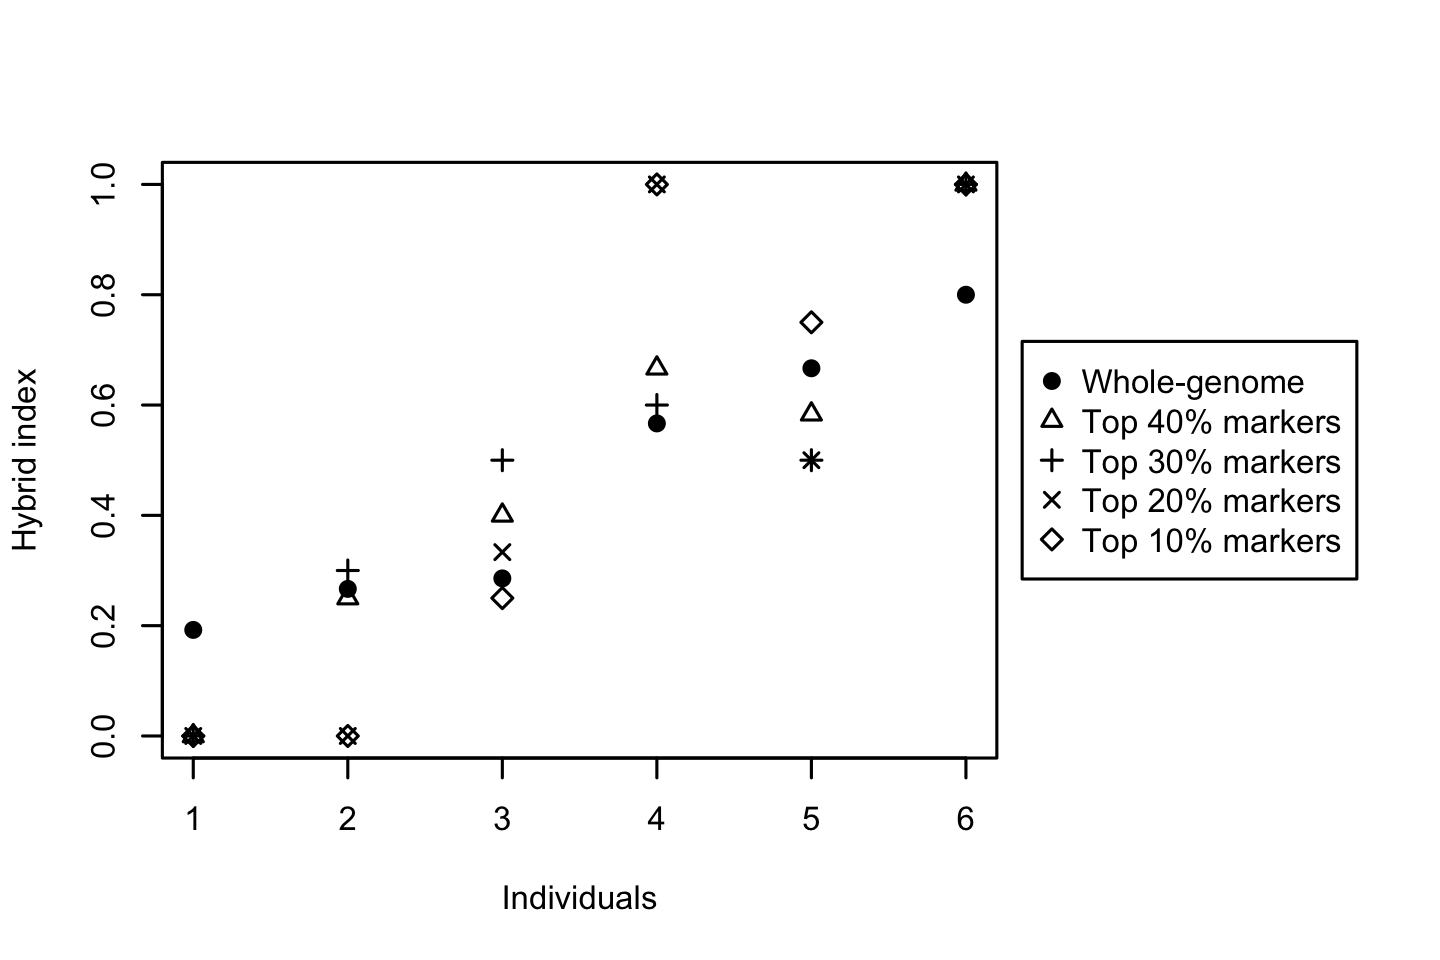
\includegraphics[width=1\linewidth]{figs/HI}

Based on these plots, the barrier to gene flow progressively increases. Note that the order of individuals was taken from \emph{the HIwithOptimalPolarities.txt} file produced by the \texttt{diem} run. These values are based on whole-genome variability taking into account compartment ploidy as it was defined during the analysis. This is the preferred way to explore the influence of alternative threshold values, because the visualisation is also sensitive to how individuals might change positions along the HI slope.

\textbf{Caution:} Because DI depends on allele frequency differences, sample size, and the polarities of all assessed sites, DI values are not directly comparable across independent runs, species pairs, or datasets. Derive cutoff thresholds (for example, top quantiles) within each dataset, and report the number or proportion of retained markers.

\section{Biological signal insights}\label{biological-signal-insights}

Filtering by DI is not mandatory, but it is an efficient way to reveal the core signal of genome polarisation. Patterns that were previously noisy or ambiguous often become clear once low‑information markers are excluded. When reporting results, state your DI quantile cutoff and confirm that qualitative interpretations remain robust across reasonable thresholds.

Diagnostic markers often occur in genomic regions under strong differentiation or selection that maintain alternative alleles between taxa, whereas sites with low diagnostic index are typically typically reflect shared or neutral polymorphisms. Thus, filtering sites by diagnostic index not only increases contrast but also enriches for genomic regions that maintain species boundaries.

Because markers with high DI are not evenly distributed along chromosomes \citep{Jagos2025}, DI filtering can shift the apparent contribution of different genomic regions to the overall signal. Regions with many fixed differences will remain densely represented, while more homogeneous or highly variable regions may contribute fewer diagnostic markers. When summarising results in windows or genomic compartments, keep this unequal site density in mind.

\chapter{Smoothing polarised genotypes}\label{smoothing-polarised-genotypes}

After filtering markers by diagnostic index (Chapter \ref{DIfiltering}), genome polarisation analyses can be mapped to physical coordinates to reveal the genomic landscape of barriers to gene flow. Because SNVs are rarely evenly spaced along chromosomes, the polarised signal can fluctuate sharply between adjacent markers. But these fluctuations might not represent signal change, but confluence with standing genetic variation. While, diagnostic index filtering already removed much of the effect of genetic variation orthogonal to the barrier to gene flow, smoothing along mapped distances helps visualise broad ancestry patterns.

\section{Smoothing across mapped distances}\label{smoothing-across-mapped-distances}

The \texttt{smoothPolarizedGenotypes} function applies kernel smoothing to the polarised genotype matrix, using physical distances between markers rather than their rank order. This approach preserves the broad genomic signal while suppressing local irregularities caused by uneven SNV spacing.

\subsection{Mapping diagnostic markers}\label{mapping-diagnostic-markers}

The chromosomal coordinates of diagnostic markers are stored in the output file \emph{-includedSites.txt}, created during VCF conversion by the function \texttt{vcf2diem}. This file lists all sites retained for polarisation and includes columns CHROM, POS, QUAL from the VCF file and allele0 and allele2 indicating alleles represented by the respective numbers when homozygous.

The positional information needed for smoothing can be extracted directly from this file. The function \texttt{rank2map} converts the ranked order of sites in the polarised genotype matrix into their corresponding chromosomal coordinates based on the *-includedSites.txt file. While it is called internally by \texttt{smoothPolarizedGenotypes}, exploring its output helps understand how physical mapping guides the smoothing process.

Full code to prepare data to execute the examples in this chapter

\begin{Shaded}
\begin{Highlighting}[]
\FunctionTok{library}\NormalTok{(diemr)}

\NormalTok{dat }\OtherTok{\textless{}{-}} \FunctionTok{system.file}\NormalTok{(}\StringTok{"extdata"}\NormalTok{, }\StringTok{"myotis.vcf"}\NormalTok{, }\AttributeTok{package =} \StringTok{"diemr"}\NormalTok{)}

\FunctionTok{vcf2diem}\NormalTok{(}\AttributeTok{SNP =}\NormalTok{ dat, }\AttributeTok{filename =} \StringTok{"myo"}\NormalTok{, }\AttributeTok{requireHomozygous =} \ConstantTok{FALSE}\NormalTok{)}

\FunctionTok{set.seed}\NormalTok{(}\DecValTok{54869}\NormalTok{)}
\NormalTok{res }\OtherTok{\textless{}{-}} \FunctionTok{diem}\NormalTok{(}\StringTok{"myo{-}001.txt"}\NormalTok{, }\AttributeTok{ChosenInds =} \DecValTok{1}\SpecialCharTok{:}\DecValTok{14}\NormalTok{)}

\NormalTok{gen }\OtherTok{\textless{}{-}} \FunctionTok{importPolarized}\NormalTok{(}\StringTok{"myo{-}001.txt"}\NormalTok{, }
  \AttributeTok{changePolarity =}\NormalTok{ res}\SpecialCharTok{$}\NormalTok{markerPolarity, }
  \AttributeTok{ChosenInds =} \DecValTok{1}\SpecialCharTok{:}\DecValTok{14}  
\NormalTok{)}

\NormalTok{HI }\OtherTok{\textless{}{-}} \FunctionTok{hybridIndex}\NormalTok{(gen)}
\end{Highlighting}
\end{Shaded}

\begin{Shaded}
\begin{Highlighting}[]
\CommentTok{\# read the includedSites file}
\NormalTok{bed }\OtherTok{\textless{}{-}} \FunctionTok{readIncludedSites}\NormalTok{(}\StringTok{"myo{-}includedSites.txt"}\NormalTok{)}

\CommentTok{\# generate mapping of ranks to genome positions}
\NormalTok{windows }\OtherTok{\textless{}{-}} \FunctionTok{rank2map}\NormalTok{(}\StringTok{"myo{-}includedSites.txt"}\NormalTok{, }\AttributeTok{windowSize =} \DecValTok{150}\NormalTok{)}

\CommentTok{\# show how window ranges correspond to sites}
\FunctionTok{cbind}\NormalTok{(windows, bed)}
\CommentTok{\#     1  2      CHROM POS QUAL allele0 allele2}
\CommentTok{\# 1   1  1 KE210828.1  60    .       A       G}
\CommentTok{\# 2   2  2 KE210828.1 171    .       G       T}
\CommentTok{\# 3   3  3 KE212673.1  84    .       A       T}
\CommentTok{\# 4   4  4 KE214857.1  90    .       A       G}
\CommentTok{\# 5   5  8 KE222443.1 134    .       G       A}
\CommentTok{\# 6   5  8 KE222443.1 156    .       T       G}
\CommentTok{\# 7   5  9 KE222443.1 171    .       T       G}
\CommentTok{\# 8   5  9 KE222443.1 183    .       C       T}
\CommentTok{\# 9   7  9 KE222443.1 244    .       C       G}
\CommentTok{\# 10 10 10 KE222801.1 100    .       G       A}
\CommentTok{\# 11 11 14 KE224361.1 120    .       G       A}
\CommentTok{\# 12 11 14 KE224361.1 132    .       G       C}
\CommentTok{\# 13 11 14 KE224361.1 175    .       A       C}
\CommentTok{\# 14 11 14 KE224361.1 179    .       G       T}
\CommentTok{\# 15 15 15 KE227386.1 153    .       A       G}
\end{Highlighting}
\end{Shaded}

Each entry in \texttt{windows} corresponds to one marker in the \emph{myo-includedSites.txt} file and shows a range of sites that are within the desired \texttt{windowSize}, where the window is centered at the reference site. In practice, \texttt{rank2map} looks for half the \texttt{windowSize} in either direction from the evaluated site, respecting the afinity to unique \texttt{CHROM} values. For genomes composed of multiple scaffolds or chromosomes, smoothing should be performed separately for each element, and \texttt{rank2map} ensures that the windows are set up with respect to \texttt{CHROM} values.

\subsection{Visual comparison of raw and smoothed results}\label{visual-comparison-of-raw-and-smoothed-results}

For smoothing to work, the sites in the original vcf file must be sorted.

\begin{Shaded}
\begin{Highlighting}[]
\CommentTok{\# smooth the polarised genotypes using a 150 bp window}
\NormalTok{genSmooth }\OtherTok{\textless{}{-}} \FunctionTok{smoothPolarizedGenotypes}\NormalTok{(}\AttributeTok{genotypes =}\NormalTok{ gen,}
    \AttributeTok{includedSites =} \StringTok{"myo{-}includedSites.txt"}\NormalTok{,}
    \AttributeTok{windowSize =} \DecValTok{150}\NormalTok{)}
\end{Highlighting}
\end{Shaded}

The object returned by \texttt{smoothPolarizedGenotypes} is a genotype matrix with the same dimensions and site order as the input but containing smoothed genomic state values. These can be used interchangeably with raw genotypes in visualisation and hybrid index calculations.

The smoothing window is expressed in base pairs, should correspond to the expected local scale of linkage. As recombination rates differ among taxa, selecting an appropriate window is best guided by empirical inspection. Compare several values to find the level of smoothing that preserves broad ancestry patterns without obscuring fine-scale transitions.
Larger windows produce a more continuous signal but can merge distinct ancestry blocks, while smaller windows follow local fluctuations more closely. The optimal setting depends on marker density and linkage along the genome.

Smoothing is recommended only for mapped data. Applying it to unordered or scaffold-level data can distort the genomic signal.

Smoothing does not change the overall polarity of sites but modifies their local continuity. The following example compares raw and smoothed genotypes.

\begin{Shaded}
\begin{Highlighting}[]
\FunctionTok{par}\NormalTok{(}\AttributeTok{mfrow =} \FunctionTok{c}\NormalTok{(}\DecValTok{1}\NormalTok{, }\DecValTok{2}\NormalTok{))}
\FunctionTok{plotPolarized}\NormalTok{(gen, HI)}
\FunctionTok{plotPolarized}\NormalTok{(genSmooth, HI)}
\end{Highlighting}
\end{Shaded}

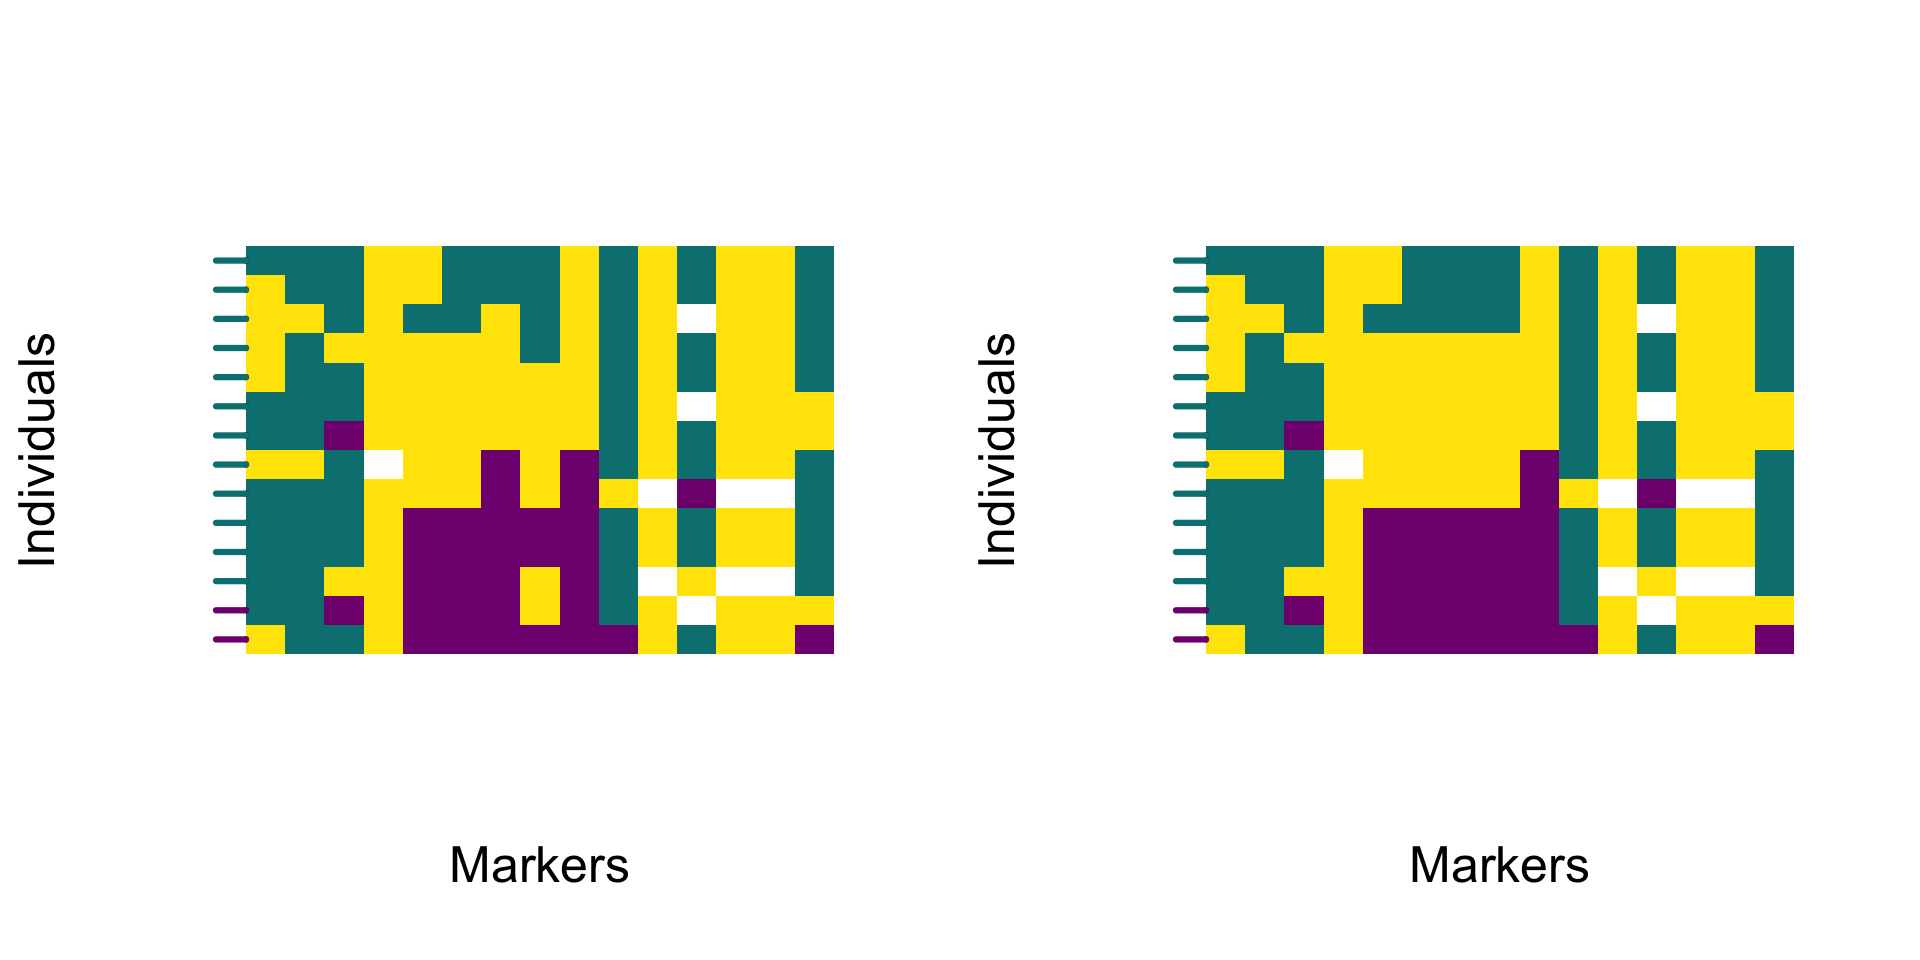
\includegraphics[width=1\linewidth]{figs/smooth}

The smoothed profile follows the same overall trajectory as the raw data but removes short-range noise caused by individual SNVs. The resulting heatmap highlights broad transitions in ancestry and provides a clearer estimate of barrier to gene flow along chromosomes.

\section{Interpretation and downstream use}\label{interpretation-and-downstream-use}

Smoothing algorithm implemented in \texttt{diemr} since version 1.4.2 uses a truncated Laplace kernel to calculate weighted mode genomic state for each smoothed site. The Laplace kernel gives the highest weight to nearby markers while gradually down-weighting distant ones, producing smooth but localised transitions in the polarised signal. The truncation limits the influence of distant loci so that ancestry shifts remain aligned with finite physical genomic distance.

Mapping and smoothing improve interpretability of \emph{diem} output in three ways:

\begin{enumerate}
\def\labelenumi{\arabic{enumi}.}
\item
  stabilising local genomic states and reducing noise caused by marker spacing,
\item
  expressing barrier strength and ancestry transitions in physical coordinates, and
\item
  facilitating integration with genomic context such as recombination rate, gene density, or structural features.
\end{enumerate}

When reporting smoothed results, always specify the window size and kernel type used.
Smoothing clarifies broad-scale patterns but should not replace marker-level interpretation.

\textbf{Methodological explanation of the Laplace kernel smoothing}

\subsection{Methodological explanation of the Laplace kernel smoothing}\label{methodological-explanation-of-the-laplace-kernel-smoothing}

The smoothing algorithm applies a truncated Laplace kernel over physical distance and assigns each site the weighted modal genomic state within the window. This can be described as \textbf{Laplace-kernel weighted mode smoothing}.

Smoothing is applied \textbf{per chromosome}. For each individual \(i\) and focal site \(j\) at position \(x_j\), we consider all neighbouring sites within a symmetric window of half-width \(\text{windowSize}/2\) base pairs. Rather than averaging genotype values, the algorithm computes a \textbf{kernel-weighted vote} over discrete genomic states \(s \in {0,1,2}\) (homozygous genotypes of two most frequent alleles denoted as \texttt{0} and \texttt{2}, and heterozygots as \texttt{1}, chapter \ref{diemFormat}) and assigns the \textbf{state with the highest weighted support} to the focal site.

The goal is to reduce short-range noise caused by uneven marker spacing and stochastic variation, while preserving discrete genomic states that reflect linkage blocks and recombination.

The smoothing method considers a \textbf{centred physical window} of width \texttt{windowSize} (bp), i.e.~positions \(x\) with
\[
x \in \left[x_j - \frac{\text{windowSize}}{2}, x_j + \frac{\text{windowSize}}{2}\right].
\]
Within that window, neighbouring markers ``vote'' for their discrete genomic states \(s\in{0,1,2}\) with \textbf{Laplace weights} that decay with distance from the focal site. The smoothed value at \(j\) is the \textbf{weighted mode} (state with the largest total weight).

It is important that the smoothing is applied to physical distances between SNVs, so the \texttt{rank2map} internally computes the \textbf{start and end site indices} whose positions fall inside the centred interval for site \(j\).

\subsubsection{Implemented kernel, truncation and scaling}\label{implemented-kernel-truncation-and-scaling}

Let \(d = x - x_j\) be the \textbf{centred physical distance} (bp) from the focal site. The kernel is only ever evaluated inside the centred window; weights for positions outside are never computed or used.

Define the \textbf{Laplace scale} \(b\) as a function of \texttt{windowSize}:
\[
b = \frac{\text{windowSize}}{2 \ln 20}.
\]

This choice guarantees that a two-sided Laplace distribution truncated at \(\pm b\ln 20\) retains 95\% of its mass (because \(\Pr(|X|>a)=e^{-a/b}\), so with \(a=b\ln 20\), the tail is \(1/20=0.05)\).

The code evaluates integer-spaced centred offsets
\[
x \in {-\lfloor \tfrac{\text{windowSize}}{2}\rfloor,\ldots, -1,0,1,\ldots,\lfloor \tfrac{\text{windowSize}}{2}\rfloor}
\]
and assigns \textbf{truncated Laplace weights}:
\[
w_x = \frac{10}{19} \exp\left(-\frac{|x|}{b}\right),\quad \text{for } |x| \le \frac{\text{windowSize}}{2}.
\]

\begin{quote}
\textbf{Notes on scaling and normalisation:}

\begin{itemize}
\tightlist
\item
  The constant \(10/19\) is an explicit global scaling applied to all in-window weights (see \texttt{truncatedLaplace}); it is not a per-site normalisation.
\item
  Because the algorithm selects a \textbf{weighted mode}, only relative weights matter; any common multiplicative constant cancels.
\item
  There is no per-window re-normalisation; the code compares \textbf{sums of weights} across states directly.
\end{itemize}
\end{quote}

\subsubsection{Weighted-mode smoothing}\label{weighted-mode-smoothing}

For each focal site \(j\) and individual \(i\), we compute \textbf{state-specific support} by summing weights over all neighbours within the centred window whose genotype equals that state:
\[
S_s(i,j) = \sum_{k \in \text{window}(j)}
  \begin{cases}
    w_{(x_k - x_j)}, & \text{if } g_{i,k} = s, \\
    0, & \text{otherwise.}
  \end{cases}
\]

The \textbf{smoothed state} is the argmax:
\[
\tilde g_{i,j} = \arg\max_{s\in{0,1,2}} S_s(i,j),
\]
ignoring \texttt{NA} genotypes in the sums.

\subsubsection{Tie-breaking (exact order used)}\label{tie-breaking-exact-order-used}

If two or more states tie, internal function \texttt{unbiasedWeightedStateChoice} breaks ties in this strict sequence:

\begin{enumerate}
\def\labelenumi{\arabic{enumi}.}
\tightlist
\item
  \textbf{Higher total weight} \(S_s(i,j)\) (the primary criterion).
\item
  \textbf{Higher single-occurrence weight} for the state (i.e.~the largest \(w\) among markers supporting that state).
\item
  \textbf{Lexicographic order} of the state label (with numeric states treated as character, effectively \texttt{"0"\ \textless{}\ "1"\ \textless{}\ "2"}).
\end{enumerate}

This is the complete list; there is \textbf{no} preference for the focal site's own genotype unless it wins under the rules above.

  \bibliography{refs.bib}

\end{document}
